Candidate events are required to have at least a reconstructed $pp$ interaction vertex with at least two $\pt > 400$~{\MeV} associated tracks.
The vertex with the largest $\sum \pt^{2}$ of the associated tracks is selected as the primary vertex of the event. 
In this chapter, the various object reconstructions and  identifications in the ATLAS experiment are presented.
The electron, muon, and tau objects are presented in Sect.~\ref{subsec:event_electrons},~\ref{subsec:event_muons}, and~\ref{subsec:event_Taus}, respectively.
Followed by the photons in Sect.~\ref{subsec:event_photons}, jets in Sect.~\ref{subsec:event_jets}, and \met in Sect.~\ref{subsec:event_met}.
Finally, the signal region (SR) selection is described in Sect.~\ref{sec:event_signal_region_selection}.

%%%
%%%
%%%

\section{Object selections}
\label{sec:event_object_selections}
This section presents the object definition and selection in the analysis.
The general object selections for ATLAS are described followed by the specific selections used for this analysis.
The definition of objects used in this analysis are based on the recommendations by Combined Performance groups and are summarized in Table~\ref{tab:event_object_definitions}.
The objects are divided into two categories: preselected and signal objects where signal objects are a subset of preselected objects.
Unless otherwise stated, the recommendations implemented in \texttt{SUSYTools-00-08-69}~\cite{SUSYToolsV8} and \texttt{AnalysisBase 2.4.37}~\cite{AnalysisBase} are used for all the objects.

\begin{table}[ht]
    \begin{center}
        {\scriptsize
            \begin{tabular}{lll}
                \hline
                \hline
                Property           & Preselected object                     & Signal object\\
                \hline
                \textbf{Electrons} &                                        &\\
                Kinematic          & $\pt > 4.5$~{\GeV}                     & $\pt > 4.5$~{\GeV}, $|\eta| < 2.47$ (include crack)\\
                Identification     & \texttt{VeryLooseLLH}                  & \texttt{TightLLH}\\
                Isolation          & -                                      & \texttt{GradientLoose}\\
                Impact parameter   & $|z_{0} \sin\theta| < 0.5$~mm          & $|d_{0}/\sigma(d_{0})| < 5$, $|z_{0} \sin\theta| < 0.5$~mm\\
                Reco algorithm     & Veto \texttt{author==16}               & Veto \texttt{author==16}\\
                \hline
                \textbf{Muons}     &                                        &\\
                Kinematic          & $\pt > 4$~{\GeV}                       & $\pt > 4$~{\GeV}, $|\eta| < 2.5$\\
                Identification     & \texttt{Medium}                        & \texttt{Medium}\\
                Isolation          & -                                      & \texttt{FixedCutTightTrackOnly}\\
                Impact parameter   & $|z_{0} \sin\theta| < 0.5$~mm          & $|d_{0}/\sigma(d_{0})| < 3$, $|z_{0} \sin\theta| < 0.5$~mm\\
                \hline
                \textbf{Jets}
                Kinematic          & $\pt > 20$~{\GeV}, $|\eta| < 4.5$      & $\pt > 30$~{\GeV}, $|\eta| < 2.8$\\
                Clustering         & Anti-$k_{t}$ $R = 0.4$ \texttt{EMTopo} & Anti-$k_{t}$ $R = 0.4$ \texttt{EMTopo}\\
                Pileup mitigation  & -                                      & JVT \texttt{Medium} for $\pt < 60$~{\GeV}, $|\eta| < 2.4$\\
                $b$-tagging        & -                                      & $\pt > 20$~{\GeV}, $|\eta| < 2.5$, \texttt{MV2c10} \texttt{FixedCutBeff} 85\%\\
                \hline
                \hline
            \end{tabular}
        }
    \end{center}
    \caption{Summary of objec definitions used in this analysis.}
    \label{tab:event_object_definitions}
\end{table}%

%%%
%%%
%%%

\subsection{Electrons}
\label{subsec:event_electrons}

%%%
%%%
%%%

\subsubsection{General electron reconstruction and identification}
\label{subsubsec:event_electrons_general}
In the ATLAS experiment, electron\footnote{Electrons and positrons are collectively referred to as electrons.} objects are reconstructed and identified using the information from the ID tracks matched to energy clusters in the ECAL.
Electron candidates with $\pt > 4$~{\GeV} and $|\eta| < 2.47$ are selected using the tag-and-probe method for $Z \to ee$ and $J/\psi \to ee$ processes.
Three likelihood based electron identification algorithms, \texttt{Loose}, \texttt{Medium}, and \texttt{Tight} are applied to determine the signal-like reconstructed electron candidates.
These three identifications use the same variables to define the likelihood discriminant but with different selection criteria.
Depending on the electron identification used, the reconstruction efficiency varies from 78 to 90\% and increases with \met.
The electron isolation varies between 90\% and 99\% depending on the isolation selection criteria.
More detail about the electron reconstruction performance can be found in Ref.~\cite{ATLAS:2016iqc} and a detail description about the electron isolation, which is my authorship project, can be found in the App.~\ref{app:electron_isolation}.

%%%
%%%
%%%

\subsubsection{Specific to this analysis}
\label{subsubsec:event_electrons_specific}
The preselected electrons used in this analysis have to satisfy $\pt > 4.5$~{\GeV} and $|\eta| < 2.47$ and pass the likelihood-based \texttt{VeryLooseLLH} identification.
The electron tracks are required to satisfy the longitudinal impact parameter $|z_{0}\sin\theta| < 0.5$~mm.
The electrons coming from the photon conversion are rejected by veto the \texttt{author==16}.
The signal electrons have a tighter selection criteria.
Besides all the requirements for the preselected electrons, the signal electrons are also required to pass \texttt{TightLLH} identification, \texttt{GradientLoose} isolation, and the transverse impact parameter $|d_{0}/\sigma(d_{0})| < 5$ requirements.

%%%
%%%
%%%

\subsection{Muons}
\label{subsec:event_muons}

%%%
%%%
%%%

\subsubsection{General muon reconstruction and identification}
\label{subsubsec:event_muons_general}
In the ATLAS experiment, muon objects are reconstructed and identified using the information from ID and muon spectrometer in the $\pt > 4$~{\GeV} and $|\eta| < 2.7$ region.
Muon candidates are identified by applying quality requirements to suppress background which mainly come from pion and kion decays.
Four categories of muon identification, \texttt{Medium}, \texttt{Loose}, \texttt{Tight}, and \texttt{High}-\pt are provided for different physics analyses.
The \texttt{Medium} minimizes the systematic uncertainties and is provided as the default selection for muons in ATLAS.
The \texttt{Loose} maximize the reconstruction efficiency and is used for multilepton final state analyses.
The \texttt{Tight} maximize the purity of muons and the \texttt{High}-\pt maximize the momentum resolution for $\pt > 100$~{\GeV}.
The muon reconstruction efficiency is about 99\% in $5 < \pt < 100$~{\GeV} and $|\eta| < 2.5$ phase space.
The muon isolation efficiency varies between 93\% and 100\% depending on the isolation selection criteria.
More detail about the muon reconstruction performance can be found in Ref.~\cite{Aad:2016jkr}.

%%%
%%%
%%%

\subsubsection{Specific to this analysis}
\label{subsubsec:event_muons_specific}
%Similar to the preselected electrons, the preselected muons are reconstructed by combining the tracks information from ID and the muon spectrometer.
The preselected muons used in this analysis have to satisfy $\pt > 4$~{\GeV} and $|\eta| < 2.5$, pass the \texttt{Medium} identification, and require $|z_{0}\sin\theta| < 0.5$~mm on the longitudinal impact parameter.
A tighter requirement is applied on the signal muons which in addition pass the \texttt{FixedCutTightTrackOnly} isolation together with $|d_{0}/\sigma(d_{0})| < 3$ on the transverse impace parameter.

%%%
%%%
%%%

\subsection{Taus}
\label{subsec:event_Taus}

%%%
%%%
%%%

\subsubsection{General $\tau$ reconstruction and identification}
\label{subsubsec:event_taus_general}
The mass of $\tau$ lepton is 1.77~{\GeV} and the decay length is 80~$\mu$m which is too short to make $\tau$ reaches the active region of the ATLAS detector.
The $\tau$ can decay either leptonically ($\tau \to \ell \nu_{\ell}$, $\ell = e, \mu$) or hadronically ($\tau \to$ hadrons + $\nu_{\tau}$).
The hadronic tau decays are about 65\% of all possible decay modes and the decay products contain one charged pions (22\%) or three charged pions (72\%) of all cases.
Tau candidates are seeded by jets using the method described in Ref.~\cite{ATLAS:2017mpa} and they are required to have $\pt > 10$~{\GeV} and $|\eta| < 2.5$ but veto the candidates in the crack region $1.37 < |\eta| < 1.52$.
A boosted decision tree (BDT) based algorithm is used to identify the $\tau$ candidate and to reject backgrounds from quark- and gluon-initiated jets.
Three identifications, \texttt{Loose}, \texttt{Medium}, and \texttt{Tight} are provided with the efficiency 60\%, 55\%, and 45\% for 1-track and 50\%, 40\%, and 30\% for 3-tracks, respectively.
More detail about the $\tau$ lepton reconstruction and identification performance can be found in Ref.~\cite{ATLAS:2017mpa}.

%%%
%%%
%%%

\subsubsection{Specific to this analysis}
\label{subsubsec:event_taus_specific}
The di-tau invariant mass $m_{\tau\tau}$ is used in this analysis and addressed in Sect.~\ref{subsec:event_discriminating_variables}.

%%%
%%%
%%%

\subsection{Photons}
\label{subsec:event_photons}

%%%
%%%
%%%

\subsubsection{General photons reconstruction and identification}
\label{subsubsec:event_photons_general}
In the ATLAS experiment, photons are reconstructed using the tracking information in ID and the energy deposits in the CAL.
To distinguish prompt photons\footnote{Prompt photons are photons not originating from hadron decays} from background photons, the photon identification is based on a set of rectangular cuts on several discriminating variables computed from the energy deposited in the ECAL and from the shower leakage to the HCAL.
The photon identification is separately applied to the converted and unconverted photons with $25 \le E_{\mathrm{T}} \le 1500$~{\GeV} and 4 $|\eta|$ intervals.
Two identifications, \texttt{Loose} and \texttt{Tight}, are provided.
The \texttt{Loose} provides high efficiency with low jet rejection and the \texttt{Tight}, which is recommanded for the analyses by the Combined Performance groups, provides high fake photon rejection and good efficiency.
The \texttt{Tight} identification efficiency starts from 84\% at low $E_{\mathrm{T}}$ and reaches around 98\% in $1.37 < |\eta| < 1.81$ region for the unconverted photons.
Similar to the unconverted photons, the efficiency for the converted photons increases with energy and reaches up to 98\%.
More detail about the photon reconstruction and identification can be found in Ref.~\cite{ATLAS:2011kuc}.

%%%
%%%
%%%

\subsubsection{Specific to this analysis}
\label{subsubsec:event_photons_specific}
Photons are required to pass \texttt{Tight} identification and have $\pt > 25$~{\GeV}.

%%%
%%%
%%%

\subsection{Jets}
\label{subsec:event_jets}

%%%
%%%
%%%

\subsubsection{General jets reconstruction}
\label{subsubsec:event_jets_general}
In the ATLAS experiment, jets are reconstructed using the anti-$k_{t}$ algorithm with radius parameter $R = 0.4$.
The reconstruction algorithm uses calorimeter topological clusters in $|\eta| < 4.5$ as input.
Four jet cleaning selections, \texttt{Looser}, \texttt{Loose}, \texttt{Medium}, and \texttt{Tight}, are provided to reject the background.
The \texttt{Looser} has the highest efficiency, $\sim$99.8\%, and the \texttt{Tight} has the highest background rejection with efficiency 85\% at $\pt = 25$~{\GeV} and 98\% at $\pt > 50$~{\GeV}.
More detail about the jets reconstruction using anti-$k_{t}$ algorithm can be found in Ref.~\cite{Cacciari:2008gp}.

%%%
%%%
%%%

\subsubsection{$b$-tagging}
\label{subsubsec:event_bjets}
In the ATLAS experiment, it is very important to identify jets containing $b$ hadrons from light flavor jets\footnote{The light flavor jets mean jets containing $u$, $d$, $s$, $c$, or gluons.}.
Many $b$-tagging algorithms were developed to maintain high $b$-tagging efficiency of real $b$-jets and to retain very low misidentification efficiency of the light flavor jets.
The new developed multivariable algorithm, MV2, improving the $c$-jet rejection $\sim$40\% at 77\% $b$-tagging efficiency and the rejection power at high $b$-jet \pt is also improved.
More detail about the $b$-tagging can be found in Ref.~\cite{ATL-PHYS-PUB-2015-022, ATL-PHYS-PUB-2016-012}.

%%%
%%%
%%%

\subsubsection{Specific to this analysis}
\label{subsubsec:event_jets_specific}
The preselected jets are reconstructed with the anti-$k_{t}$ algorithm with radius parameter $R = 0.4$ and required $\pt > 20$~{\GeV} and $|\eta| < 4.5$.
Jets with $\pt < 60$~{\GeV} and $|\eta| < 2.4$ are required to satisfy \texttt{Medium} jet vertex tagger requirement which can suppress pileup jets.
The MV2c10 $b$-tagging algorithm with an 85\% efficiency is applied on the preselected jets with $|\eta| < 2.5$.
The signal jets are required to satisfy $\pt > 30$~{\GeV} and $|\eta| < 2.8$.

%%%
%%%
%%%

\subsection{Missing transverse energy}
\label{subsec:event_met}
The missing transverse energy \met is defined as the negative vector sum of \pt of all reconstructed objects including leptons, jets, and soft term as show in Eq.~(\ref{eq:event_met}).
The soft term is constructed from all tracks associated to the primary vertex but not associated with any physics object.
There two kinds of soft term, calorimeter based soft term (CST) and track based soft term (TST) are used in \met calculation.
The CST \met is constructed form the energy deposits in the CAL not associated with hard objects and the TST \met is built form ID tracks which not match to any reconstructed object.
More detail about the \met reconstruction performance can be found in Ref.~\cite{ATL-PHYS-PUB-2015-023}.
%
\begin{equation}
    \met = - (\sum \mathbf{p}_{\mathrm{T}}^{\mathrm{hard}} + \mathbf{p}_{\mathrm{T}}^{\mathrm{soft}})
    \label{eq:event_met}
\end{equation}
%

%%%
%%%
%%%

\subsection{Overlap removal}
\label{subsec:event_overlap_removal}
After preselected objects are reconstructed, an overlap removal procedure is applied to resolve ambiguities between the reconstructed jets and leptons.
The distance $\Delta R$ between two objects is used for overlap removal and $\Delta R$ is defined as
%
\begin{equation}
    \Delta R = \sqrt{(\Delta y)^{2} + (\Delta \phi)^{2}}
\end{equation}
%
where $y$ and $\phi$ are rapidity and azimuthal angle, respectively.
The overlap removal procedure has to follow the steps listed below.
In order to avoid the bremsstrahlung from muons followed by a photon conversion into electron pairs, electron candidate is reomved if it shares the same ID track with a muon object.
Jet is removed from the remaining electrons if $\Delta R(\mathrm{jets}, e) < 0.2$ unless it is a $b$-jet.
If there are less than 3 tracks of jets with $\pt > 500$~{\MeV} and the distance between jets and a muon candidate less than 0.4, i.e. $\Delta R(\mathrm{jets}, \mu) < 0.4$, then the jets are removed.
This step can suppress muon bremsstrahlung.
Finally, the electrons and muons are removed if the $e$ or $\mu$ lie in a distance $\Delta R(\mathrm{jets}, e/\mu) < 0.4$ of the surviving jets so that charm and bottom hadron decays are suppressed.

%%%
%%%
%%%

\section{Signal region selection}
\label{sec:event_signal_region_selection}

%%%
%%%
%%%

\subsection{Discriminating variables}
\label{subsec:event_discriminating_variables}
This section provides the explaniations for various variables used to discriminate signals and background.
%
\begin{itemize}
    \item \textbf{Same flavour opposite sign (SFOS) lepton pair}: This analysis requires exactly two preselected and two signal leptons in the final state.
    These two leptons have to carry the same flavor and with opposite electric charge such as $e^{\pm}e^{\mp}$ and $\mu^{\pm}\mu^{\mp}$.

    \item $\mathbf{\pt^{\ell_{1}}}$ and $\mathbf{\pt^{\ell_{2}}}$: The momentum of leading lepton $\pt^{\ell_{1}} > 5$~{\GeV} is required to suppressed fake/nonprompt leptons background and the threshold of the momentum of subleading lepton $\pt^{\ell_{2}} > 4.5$(4)~{\GeV} for electron (muon) is used to retain signal acceptance.

    \item $\mathbf{\Delta R_{\ell\ell}}$: The dilepton distance is defined as Eq.~(\ref{eq:event_dilepton_distance}).
    %This variable provides good discrimination between the Higgsino and slepton because the dileptons from Higgsinos have small angular separation.
    %However, the leptons originate from the slepton don't have strong restrictions on their angular separation.
    The $\Delta R_{\ell\ell}$ variable, which is required to greater than 0.05, suppresses the leptons originating from photon conversions or muons.
    %
    \begin{equation}
        \Delta R_{\ell \ell} = \sqrt{(\eta_{\ell_{1}} - \eta_{\ell_{2}})^{2} + (\phi_{\ell_{1}} - \phi_{\ell_{2}})^{2}}
        \label{eq:event_dilepton_distance}
    \end{equation}
    %

    \item $\mathbf{m_{\ell\ell}}$: The dilepton invariant mass $m_{\ell\ell}$ is bounded by the mass splitting $m(\widetilde{\chi}^{0}_{2}) - m(\widetilde{\chi}^{0}_{1})$ providing the background suppression power.
    The background originates from on-shell $Z$ decay can be suppressed if the upper bound of $m_{\ell\ell}$ is set to 60~{\GeV} and the contributions from $J/\psi$ are vetoed by required a $3 < m_{\ell\ell} < 3.2$~{\GeV} window.

    \item $\mathbf{\met}$: In order to keep the \met trigger efficiency exceeding 95\%, \met is required to be greater than 200~{\GeV}.

    \item $N_{\mathrm{jet}}$: The number of jets is required to greater than or equal to 1 because of the initial state radiation (ISR) jets.

    \item $\mathbf{\pt^{j_{1}}}$: The momentum of the leading jet is required to greater than 100~{\GeV}.

    \item $\mathbf{\Delta \phi(j_{1}, \pt^{\textbf{miss}})}$: The azimuthal separation between $j_{1}$ and $\mathbf{\pt^{\textrm{miss}}}$ is required to greater than 2 to suppress the QCD and $Z$+jets background.

    \item \textbf{min($\mathbf{\Delta \phi(\textbf{any jet}, \pt^{\textbf{miss}})}$)}: By requiring $\Delta \phi(\textrm{any jet}, \pt^{\textbf{miss}}) > 0.4$, the effect of jet-energy mismeasurement on \met can be reduced.

    \item $\mathbf{N}_{\mathbf{b}\textbf{-jet}}$: Requiring $N_{b\textrm{-jet}} = 0$, the \ttbar and single-top backgrounds can be reduced significantly.

    \item $\mathbf{m_{\tau\tau}}$: The di-tau invariant $m_{\tau\tau}(p_{\ell_{1}}, p_{\ell_{2}}, \mathbf{p}_{\mathrm{T}}^{\mathrm{miss}})$ variable is defined as the signed square root of $m^{2}_{\tau\tau}$.
    The $m_{\tau\tau}$ is used to reconstructed the $Z \to \tau \tau$ process where $\tau$ decays leptonically $\tau \to \ell \nu_{\ell} \nu_{\tau}$.
    Figure~\ref{fig:event_mtautau} shows the $Z$ boson leptonic decay process.
    %
    \begin{figure}[htb]
        \begin{center}
            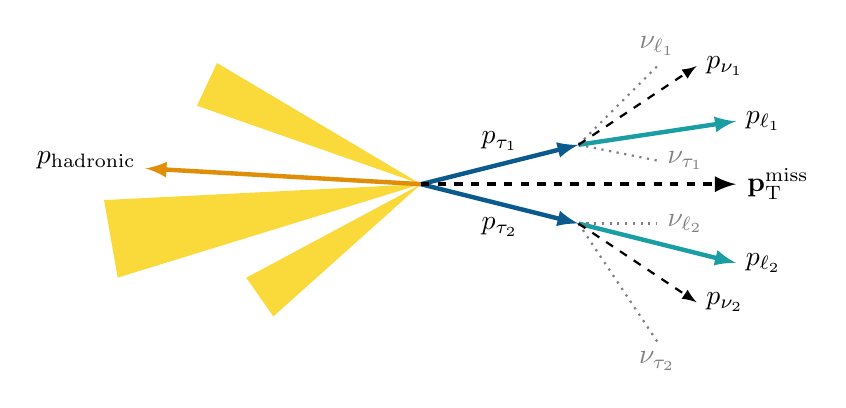
\begin{tikzpicture}

    % jets
    \definecolor{myyellow}{RGB}{249, 209, 9}
    \definecolor{myorange}{RGB}{224, 141, 8}
    \definecolor{myblue}{RGB}{11, 90, 142}
    \definecolor{mygreen}{RGB}{27, 158, 163}
    \definecolor{mylightgreen}{RGB}{186, 225, 226}
    \draw [draw=none, opacity=0.8, fill=myyellow, rotate=10] (0,0) -- (-4,-0.5)-- (-4,0.5) -- (0,0);
    \draw [draw=none, opacity=0.8, fill=myyellow, rotate=-25] (0,0) -- (-3,-0.3)-- (-3,0.3) -- (0,0);
    \draw [draw=none, opacity=0.8, fill=myyellow, rotate=35] (0,0) -- (-2.5,-0.3)-- (-2.5,0.3) -- (0,0);
    
    \draw [-latex, ultra thick, myorange] (0,0)--(-3.5,0.2);
    \node at (-3.5,0.3) [left] {$p_\mathrm{hadronic}$};
    
    % taus
    \draw [-latex, ultra thick, myblue] (0,0)--(2,0.5) ;
    \draw [-latex, ultra thick, myblue] (0,0)--(2,-0.5) ;   
    \node at (1,0.3) [above] {$p_{\tau_1}$};
    \node at (1,-0.3) [below] {$p_{\tau_2}$};
    
    % leptons
    \draw [-latex, ultra thick, mygreen] (2,0.5)--(4,0.8) ;
    \draw [-latex, ultra thick, mygreen] (2,-0.5)--(4,-1) ;      
    \node at (4,0.8) [right] {$p_{\ell_1}$};
    \node at (4,-1) [right] {$p_{\ell_2}$};
    
    % neutrinos
    \draw [dotted, thick, gray] (2,0.5) -- (3,1.5) node [above] {$\nu_{\ell_1}$};
    \draw [dotted, thick, gray] (2,0.5) -- (3,0.3) node [right] {$\nu_{\tau_1}$};
    
    \draw [dotted, thick, gray] (2,-0.5) -- (3,-2) node [below] {$\nu_{\tau_2}$};
    \draw [dotted, thick, gray] (2,-0.5) -- (3,-0.5) node [right] {$\nu_{\ell_2}$};
    
    \draw [-latex, thick, dashed] (2,0.5)--(3.5,1.5) ;
    \draw [-latex, thick, dashed] (2,-0.5)--(3.5,-1.5) ;
    \node at (3.5,1.5) [right] {$p_{\nu_1}$};
    \node at (3.5,-1.5) [right] {$p_{\nu_2}$};
    
    % MET
    \draw [-latex, ultra thick, dashed] (0,0)--(4,0) node [right] {$\mathbf{p}_\mathrm{T}^\mathrm{miss}$};
    
\end{tikzpicture}
            \caption{The illustration of the $Z \to \tau\tau$ + jets decay where $\tau$ decays leptonically $\tau \to \ell \nu_{\ell} \nu_{\tau}$.}
            \label{fig:event_mtautau}
        \end{center}
    \end{figure}
    %
    The $m^{2}_{\tau\tau}$ is defined in Eq.~(\ref{eq:event_mtautau2})
    %
    \begin{equation}
        m^{2}_{\tau\tau} \equiv 2 p_{\ell_{1}} \cdot p_{\ell_{2}} (1 + \xi_{1})(1+ \xi_{2})
        \label{eq:event_mtautau2}
    \end{equation}
    %
    where $p_{\ell_{1}}$ and $p_{\ell_{2}}$ are the momenta of the leptons and the $\xi_{1}$ and $\xi_{1}$ are the scale factor which can be determined by solving $\mathbf{p}_\mathrm{T}^\mathrm{miss} = \xi_{1} \mathbf{p}_\mathrm{T}^{\ell_{1}} + \xi_{2} \mathbf{p}_\mathrm{T}^{\ell_{2}}$.
    From the Eq.~(\ref{eq:event_mtautau2}), the $m^{2}_{\tau\tau}$ can be negative when either $1 + \xi_{1} < 0$ or $1 + \xi_{2} < 0$.
    This situation occurs when only one lepton moves in the same direction as $\mathbf{p}_{hadronic}$ and $|\mathbf{p}_{\ell}|$ is small. 
    This rarely happens for highly boosted $Z \to \tau \tau$ decays but it happens with larger frequency for less boosted heavy particles which decays back-to-back.
    The $m_{\tau\tau}$ is calculated in Eq.~(\ref{eq:event_mtautau}).
    %
    \begin{align}
        m_{\tau\tau} & = \mathrm{sign}(m^{2}_{\tau\tau}) \sqrt{|m^{2}_{\tau\tau}|}\\
                     & = 
                     \begin{cases}
                         \hphantom{-}\sqrt{m_{\tau\tau}^2}    & m_{\tau\tau}^2 \geq 0,\\
                         -\sqrt{\left| m_{\tau\tau}^2\right|} & m_{\tau\tau}^2 < 0.
                     \end{cases}
        \label{eq:event_mtautau}
    \end{align}
    %
    Despite there is a discontinuity at $m_{\tau\tau} = 0$, this variable can be used to discriminate the leptons originating from $Z\to \tau\tau$.

    \item $\mathbf{m_{T}^{\ell_{1}}}$: The transverse mass of \met and the leading lepton is defined in Eq.~(\ref{eq:event_transverse_mass}).
    The \ttbar, $WW/WZ$, and $W$+jets background can be reduced by requiring $m_{\textrm{T}}^{\ell_{1}} < 70$~{\GeV}.
    %
    \begin{equation}
        m_{\textrm{T}}^{\ell_{1}} = \sqrt{2(E_{\textrm{T}}^{\ell_{1}}\met - \mathbf{p}_{\textrm{T}}^{\ell_{1}} \cdot \mathbf{p}_{\textrm{T}}^{\textrm{miss}})}
        \label{eq:event_transverse_mass}
    \end{equation}
    %

    \item $\mathbf{\met/H_{T}^{lep}}$: The scalar sum of the lepton transverse momentum, $H_{\textrm{T}}^{\textrm{lep}}$, is defined  in Eq.~(\ref{eq:event_HT}).
    The $H_{\textrm{T}}^{\textrm{lep}}$ variable has smaller value in the compressed SUSY signal and larger value in the SM background such as $WW$ or $WZ$.
    %
    \begin{equation}
        H_{\textrm{T}}^{\textrm{lep}} = p_{\textrm{T}}^{\ell_{1}} + p_{\textrm{T}}^{\ell_{2}}
        \label{eq:event_HT}
    \end{equation}
    %
    The leptons coming from SM background, for example, \ttbar and diboson are harder but they are softer in the compressed SUSY signal events.
    Therefore, for a given value of \met, the $\met/H_{\textrm{T}}^{\textrm{lep}}$ variable is larger in the compressed signals but is smaller for the background.
    The minimal requirement of this variable is defined in Eq.~(\ref{eq:event_METOverHT}) which is adjusted event by event depending on the mass splitting.
    %
    \begin{equation}
        \met/H_{\textrm{T}}^{\textrm{lep}} > \mathrm{max}[5, 15 - 2 m_{\ell\ell}/(1~{\GeV})]
        \label{eq:event_METOverHT}
    \end{equation}
    %
    Figure~\ref{fig:event_METOverHT} shows the $\met/H_{\textrm{T}}^{\textrm{lep}}$ requirement for the electroweakino SR after applying all the SR common requirements and the $\Delta R_{\ell\ell} < 2$.
    %
    \begin{figure}[htb]
        \begin{center}
            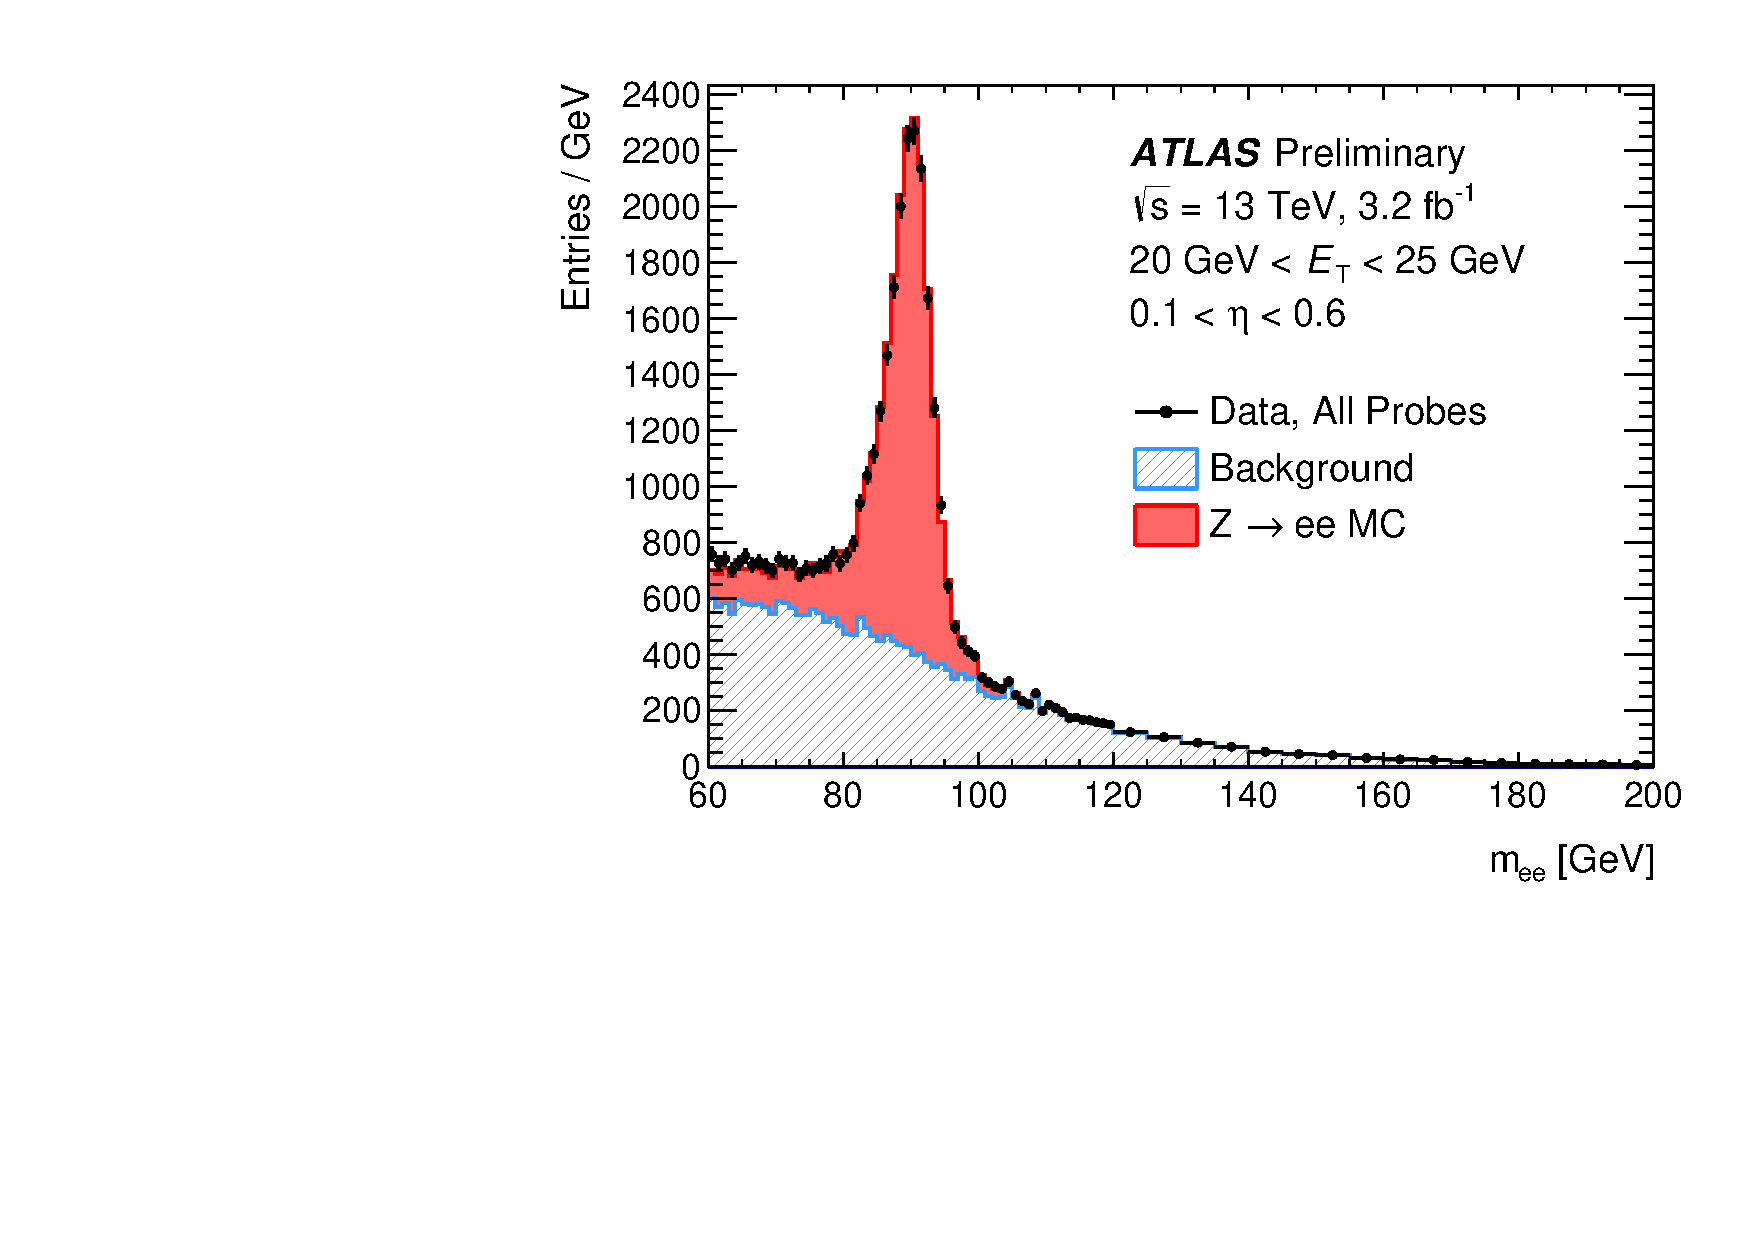
\includegraphics[scale=0.5]{fig_03a.pdf}
            \caption{The distribution of $\met/H_{\textrm{T}}^{\textrm{lep}}$ as function of $m_{\ell\ell}$ for the electroweakino after applying all the SR common requirements and the $\Delta R_{\ell\ell} < 2$.
            The red line indicates the SR selection.
            Events in the region below this line are rejected.
            The signal events are labled in colored circles for different mass splitting.}
            \label{fig:event_METOverHT}
        \end{center}
    \end{figure}
    %
\end{itemize}
%

%%%
%%%
%%%

\subsection{Signal region}
\label{subsec:event_signal_region}
The events with 2 lepton final state are selected if the lepton pair satisfies same flavor and opposite charge (SFOS).
To optomize the signal selection criteria, a number of scans over the cut values of discriminating variables listed in Sect.~\ref{subsec:event_discriminating_variables} are performed and the significance $Z_{n}$ is calculated.
In order to maximizing the $Z_{n}$, an integrated luminosity of 36~\ifb and a systematic uncertainty of 20\% on the background are assumed and at least one background event remaining is required after optimized cuts . 
A set of binned dilepton invariant mass $m_{\ell \ell}$ are defined in SR and the kinematic distribution of $m_{\ell \ell}$ is used in a fit to extract the number of signal events.
The event selection criteria for the SR are summarized in Table~\ref{tab:event_signal_region} and the $m_{\ell\ell}$ binnings are listed in Table~\ref{tab:event_signal_region_binning}.
There are 14 exclusive regions and 7 inclusive regions are defined.
The exclusive regions are used to set model-dependent limits while the inclusive regions are used to set the model-independent upper limits.
When derive the exclusion limits on the signal model, the SR$ee$-$m_{\ell\ell}$ and SR$\mu\mu$-$m_{\ell\ell}$ regions are combined and fit simultaneously.
The tightest inclusive region allows the mass splitting 1 $\sim$ 3~{\GeV} is the most compressed scenario while the looser regions allow large mass splitings up to 60~{\GeV}.

\begin{table}[htb]
    \begin{center}
        {\scriptsize
            \begin{tabular}{ll}
                \hline
                \hline
                Variable                                                               & Common requirement\\
                \hline
                Number of leptons                                                      & = 2\\
                Lepton charge and flavor                                               & $e^{+}e^{-}$ or $\mu^{+}\mu^{-}$\\
                Leading lepton $\pt^{\ell_{1}}$                                        & $> 5$~{\GeV} for electron and muon\\
                Subleading lepton  $\pt^{\ell_{2}}$                                    & $> 4.5$ (4)~{\GeV} for electron (muon)\\
                $\Delta R_{\ell \ell}$                                                 & $> 0.05$\\
                $m_{\ell \ell}$                                                        & $\in$ [1, 60]~{\GeV} excluding [3.0, 3.2]~{\GeV}\\
                \met                                                                   & $> 200$~{\GeV}\\
                Number of jets                                                         & $\ge 1$\\
                Leading jet \pt                                                        & $> 100$~{\GeV}\\
                $\Delta \phi(j_{1}, \mathbf{p}^{\mathrm{miss}}_{\mathrm{T}})$          & $> 2.0$\\
                min($\Delta \phi($any jet, $\mathbf{p}^{\mathrm{miss}}_{\mathrm{T}}))$ & $> 0.4$\\
                Number of $b$-tagged jets                                              & = 0\\
                $m_{\tau \tau}$                                                        & $< 0$ or $> 160$~{\GeV}\\
                \hline
                                                                                       & Electroweakino SRs\\
                \hline
                $\Delta R_{\ell \ell}$                                                 & $< 2$\\
                $m_{T}^{\ell_{1}}$                                                     & $< 70$~{\GeV}\\
                $\met/H_{\mathrm{T}}^{\mathrm{lep}}$                                   & $>$ max(5, 15 - 2 $\frac{m_{\ell \ell}}{1~{\GeV}}$)\\
                Binned in                                                              & $m_{\ell \ell}$\\ 
                \hline
                \hline
            \end{tabular}
        }
    \end{center}
    \caption{Summary of event selection criteria.
    The upper part lists the common selection criteria and the lower part lists the SR requirement for this analysis searching electroweakinos.
    Signal leptons and signal jets are used when applying all requirements.
    The SR binning is listed in Table~\ref{tab:event_signal_region_binning}.}
    \label{tab:event_signal_region}
\end{table}%

\begin{table}[htb]
    \begin{center}
        {\scriptsize
            \begin{tabular}{lllllllll}
                \hline
                \hline
                \multicolumn{9}{c}{Electroweakino SRs}\\
                \hline
                Exclusive & SR$ee$-$m_{\ell \ell}$, SR$\mu\mu$-$m_{\ell \ell}$ & [1, 3] & [3.2, 5] & [5, 10] & [10, 20] & [20, 30] & [30, 40] & [40, 60]\\
                Inclusive & SR$\ell \ell$-$m_{\ell \ell}$                      & [1, 3] & [1, 5]   & [1, 10] & [1, 20]  & [1, 30]  & [1, 40]  & [1, 60]\\
                \hline
                \hline
            \end{tabular}
        }
    \end{center}
    \caption{The SR binnings for the electroweakino SRs.
    The SR is defined by a $m_{\ell \ell}$ range in {\GeV}.
    The exclusive bins are used to set the exclusion limits on the model and the inclusive bins are used to set the model-independent limits.}
    \label{tab:event_signal_region_binning}
\end{table}%

%%%
%%%
%%%

\subsection{Expected yields in SR}
\label{subsec:event_expected_yields_in_SR}
The expected yields in SR for the NUHM2 are estimated using the signal MC samples.
Four kind  of production channels, $\widetilde{\chi}^{0}_{2} \widetilde{\chi}^{0}_{1}$, $\widetilde{\chi}^{0}_{2} \widetilde{\chi}^{+}_{1}$, $\widetilde{\chi}^{0}_{2} \widetilde{\chi}^{-}_{1}$, and $\widetilde{\chi}^{\pm}_{1} \widetilde{\chi}^{\mp}_{1}$, and 6 different $m_{1/2}$, 350, 400, 500, 600, 700, and 800~{\GeV}, are generated.
The $\widetilde{\chi}^{0}_{2}$ decays to $\ell^{+} \ell^{-} \widetilde{\chi}^{0}_{1}$ only and $\widetilde{\chi}^{\pm}_{1}$ decays to $f\bar{f} \widetilde{\chi}^{0}_{1}$ for the $\widetilde{\chi}^{0}_{2} \widetilde{\chi}^{\pm}_{1}$ channel and to $\ell \nu_{\ell} \widetilde{\chi}^{0}_{1}$ for $\widetilde{\chi}^{\pm}_{1} \widetilde{\chi}^{\mp}_{1}$ channel.

%%%
%%%
%%%

\subsubsection{Truth level study}
\label{subsubsec:event_truth_level_study}
The truth level information in the signal MC samples are used to calculate the acceptance of the SR selection criteria.
And the expected yields after SR selection in the truth level can be obtained by taking the product of luminosity (36.1~\ifb), acceptance, filter efficiency, cross-section, and the branching ratio.
Table~\ref{tab:event_nuhm2_truth3} shows the acceptance, the cross-section, the branchings for different production channels, the 2LMET50 filter efficiency, and the expected yields in SR using the truth level information.

% Truth3 results for NUHM2
\begin{table}[htbp]
    \begin{center}
        {\tiny
            \begin{tabular}{cccccc}
                \hline
                \hline
                NUHM2 $m_{1/2}$~[{\GeV}] &                       & $\tilde{\chi}^{0}_{2}\tilde{\chi}^{0}_{1}$ & $\tilde{\chi}^{\pm}_{1}\tilde{\chi}^{\mp}_{1}$ & $\tilde{\chi}^{0}_{2}\tilde{\chi}^{+}_{1}$ & $\tilde{\chi}^{0}_{2}\tilde{\chi}^{-}_{1}$\\
                \hline
                \multirow{5}{*}{350}     & acceptance            & 0.030534                                   & 0.020215                                       & 0.017051                                   & 0.013404\\
                                         & cross-section         & 0.583519                                   & 0.954870                                       & 0.683346                                   & 0.398366\\
                                         & branching ratio       & 0.101385                                   & 0.111060                                       & 0.101385                                   & 0.101385\\
                                         & filter efficiency     & 0.22768                                    & 0.12992                                        & 0.25578                                    & 0.25287\\
                                         & expected events in SR & 14.85                                      & 10.05                                          & 10.91                                      & 4.94\\
                \hline
                \multirow{5}{*}{400}     & acceptance            & 0.032875                                   & 0.021152                                       & 0.017745                                   & 0.017960\\
                                         & cross-section         & 0.625560                                   & 0.841584                                       & 0.684520                                   & 0.397684\\
                                         & branching ratio       & 0.102935                                   & 0.111047                                       & 0.102935                                   & 0.102935\\
                                         & filter efficiency     & 0.20416                                    & 0.12201                                        & 0.22389                                    & 0.22064\\
                                         & expected events in SR & 15.60                                      & 8.71                                           & 10.11                                      & 5.85\\
                \hline
                \multirow{5}{*}{500}     & acceptance            & 0.036173                                   & 0.024281                                       & 0.023709                                   & 0.022937\\
                                         & cross-section         & 0.660309                                   & 0.728079                                       & 0.681917                                   & 0.395590\\
                                         & branching ratio       & 0.105385                                   & 0.111019                                       & 0.105385                                   & 0.105385\\
                                         & filter efficiency     & 0.17602                                    & 0.10822                                        & 0.18806                                    & 0.18924\\
                                         & expected events in SR & 15.99                                      & 7.66                                           & 11.57                                      & 6.53\\
                \hline
                \multirow{5}{*}{600}     & acceptance            & 0.042456                                   & 0.024326                                       & 0.027313                                   & 0.027153\\
                                         & cross-section         & 0.665650                                   & 0.674514                                       & 0.679145                                   & 0.393040\\
                                         & branching ratio       & 0.107604                                   & 0.110995                                       & 0.107604                                   & 0.107604\\
                                         & filter efficiency     & 0.15353                                    & 0.10002                                        & 0.16926                                    & 0.16871\\
                                         & expected events in SR & 16.85                                      & 6.57                                           & 12.19                                      & 6.99\\
                \hline
                \multirow{5}{*}{700}     & acceptance            & 0.044454                                   & 0.025197                                       & 0.031214                                   & 0.028996\\
                                         & cross-section         & 0.664327                                   & 0.643884                                       & 0.676607                                   & 0.391328\\
                                         & branching ratio       & 0.109701                                   & 0.110976                                       & 0.109701                                   & 0.109701\\
                                         & filter efficiency     & 0.13788                                    & 0.093538                                       & 0.15874                                    & 0.15801\\
                                         & expected events in SR & 16.12                                      & 6.08                                           & 13.27                                      & 7.10\\
                \hline
                \multirow{5}{*}{800}     & acceptance            & 0.043270                                   & 0.024337                                       & 0.030427                                   & 0.026019\\
                                         & cross-section         & 0.659812                                   & 0.624032                                       & 0.674869                                   & 0.390607\\
                                         & branching ratio       & 0.111643                                   & 0.110964                                       & 0.111643                                   & 0.111643\\
                                         & filter efficiency     & 0.12825                                    & 0.087180                                       & 0.14631                                    & 0.13915\\
                                         & expected events in SR & 14.75                                      & 5.30                                           & 12.11                                      & 5.68\\
                \hline
                \hline
            \end{tabular}
        }
    \end{center}
    \caption{The acceptance, the cross-section, the branchings for different production channels, the 2LMET50 filter efficiency, and the expected yields in SR common to $2\ell$ channel for four different production channels of NUHM2 signal MC samples.
    The expected yields in the SR are obtained by taking the product of luminosity (36.1~\ifb), acceptance, filter efficiency, cross-section, and the branching ratio.}
    \label{tab:event_nuhm2_truth3}
\end{table}%

%%%
%%%
%%%

\subsubsection{Kinematic distributions}
\label{subsubsec:event_kinematic_distributions}
Figure~\ref{fig:event_nuhm2_kinematic_in_SR_SFOS_1}, Fig.~\ref{fig:event_nuhm2_kinematic_in_SR_SFOS_2}, and Fig.~\ref{fig:event_nuhm2_kinematic_in_SR_SFOS_3} show the kinematic variable distributions for the NUHM2 model with $m_{1/2} = 500$~{\GeV} in $1 < \mathrm{SR}\ell \ell$-$m_{\ell \ell} < 60$~{\GeV}.
The distributions for the other $m_{1/2}$ mass points can be found in the App.~\ref{app:distributions}.
In order to compare the signal with background distributions, the NUHM2 distributions are multiplied by 10 but the number of events listed in the legend use its actual values.
When making these so called `$N-1$' plots, all the selections listed in Table~\ref{tab:event_signal_region} are applied, except the variable plotted.
The bigger arrows in the upper pad present the selection criteria of the plotting variable as listed in Table~\ref{tab:event_signal_region} and the hatched uncertainty bands in the lower pad are the quadratic sum of the statistical uncertainty and a flat 20\% systematic uncertainty on the backgrounds.

\begin{figure}[htbp]
    \begin{center}
        \begin{subfigure}[b]{0.48\textwidth}
            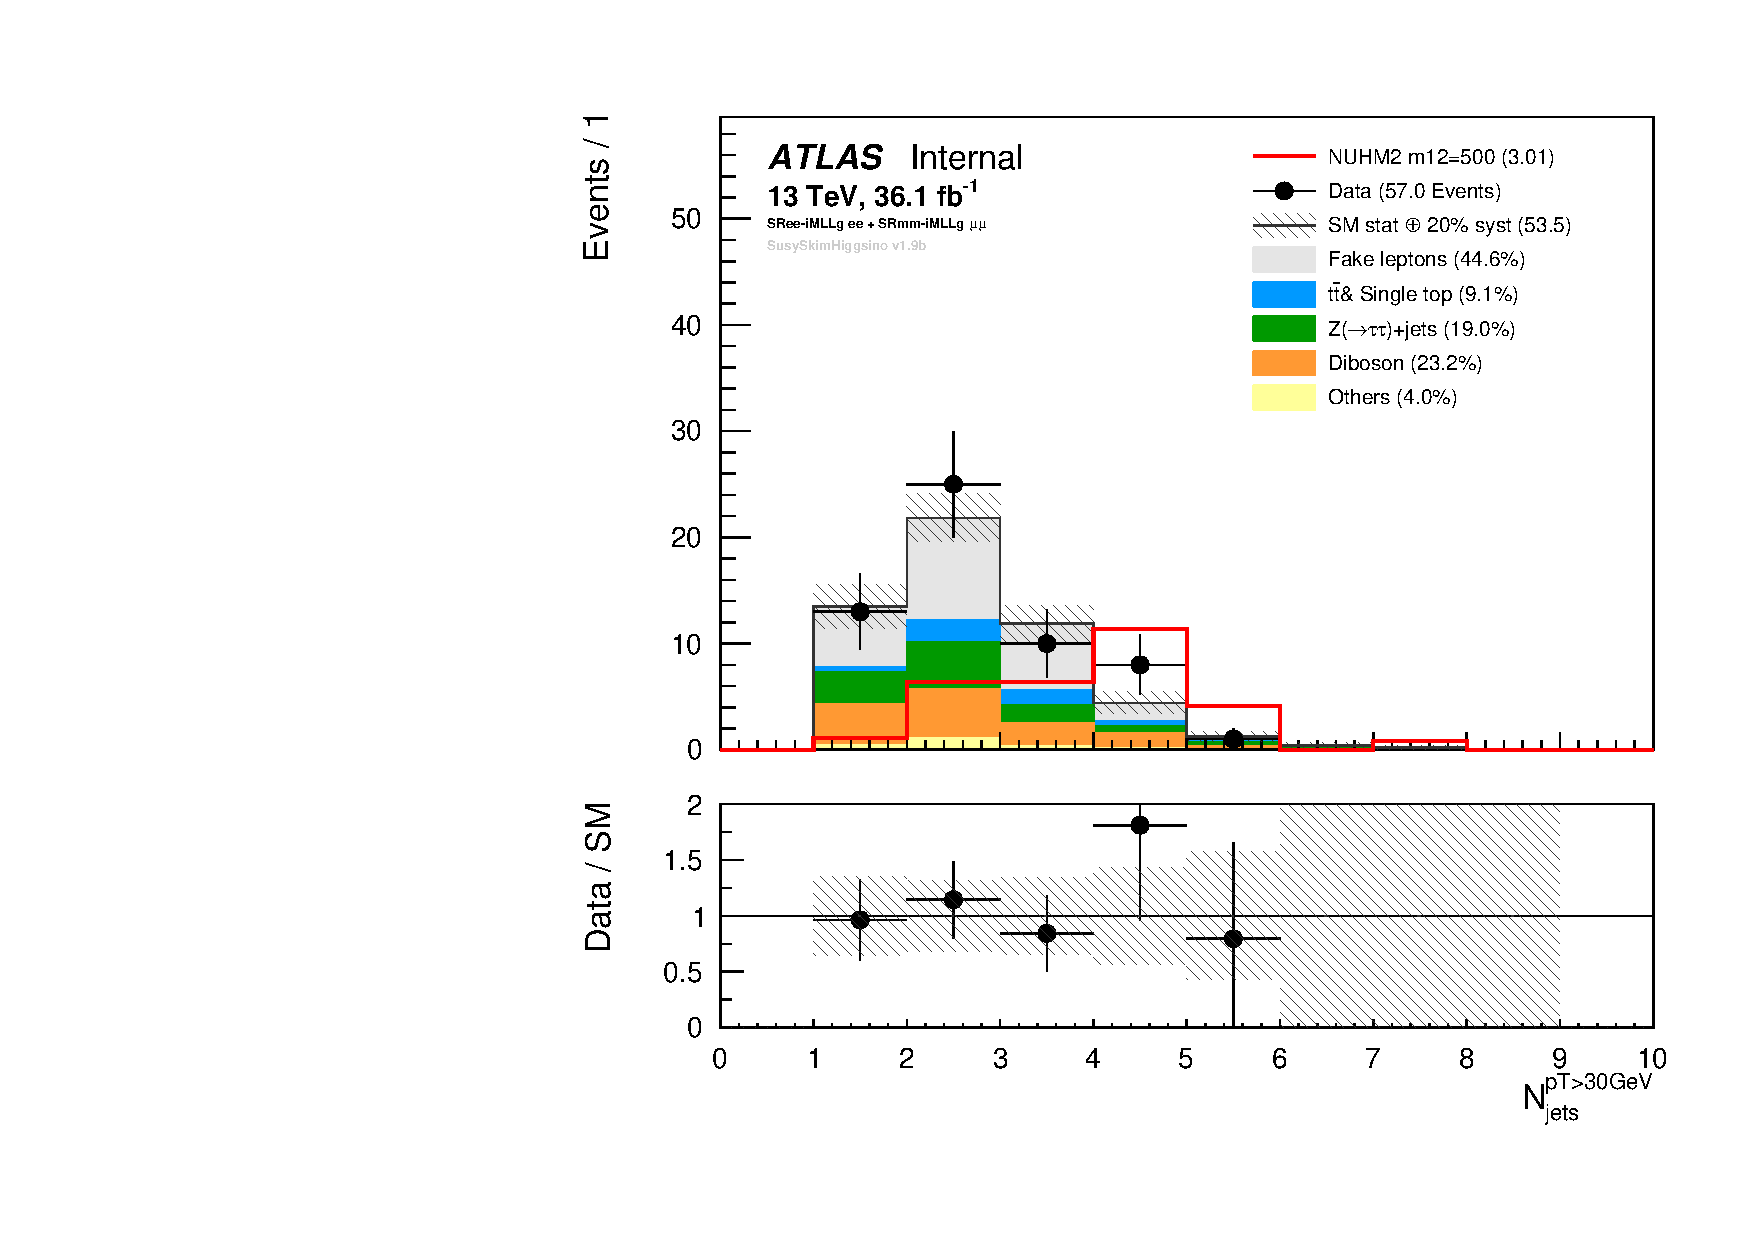
\includegraphics[scale=0.4]{NUHM2_m12_500_and_Bkg_nJet30_SFOS_N_minus_one_distribution_in_SR_times_10_on_Nsig.pdf}
            \caption{$N^{30}_{\mathrm{jets}}$}
            \label{fig:event_nuhm2_m12_500_nJet30_SFOS}
        \end{subfigure}
        \begin{subfigure}[b]{0.48\textwidth}
            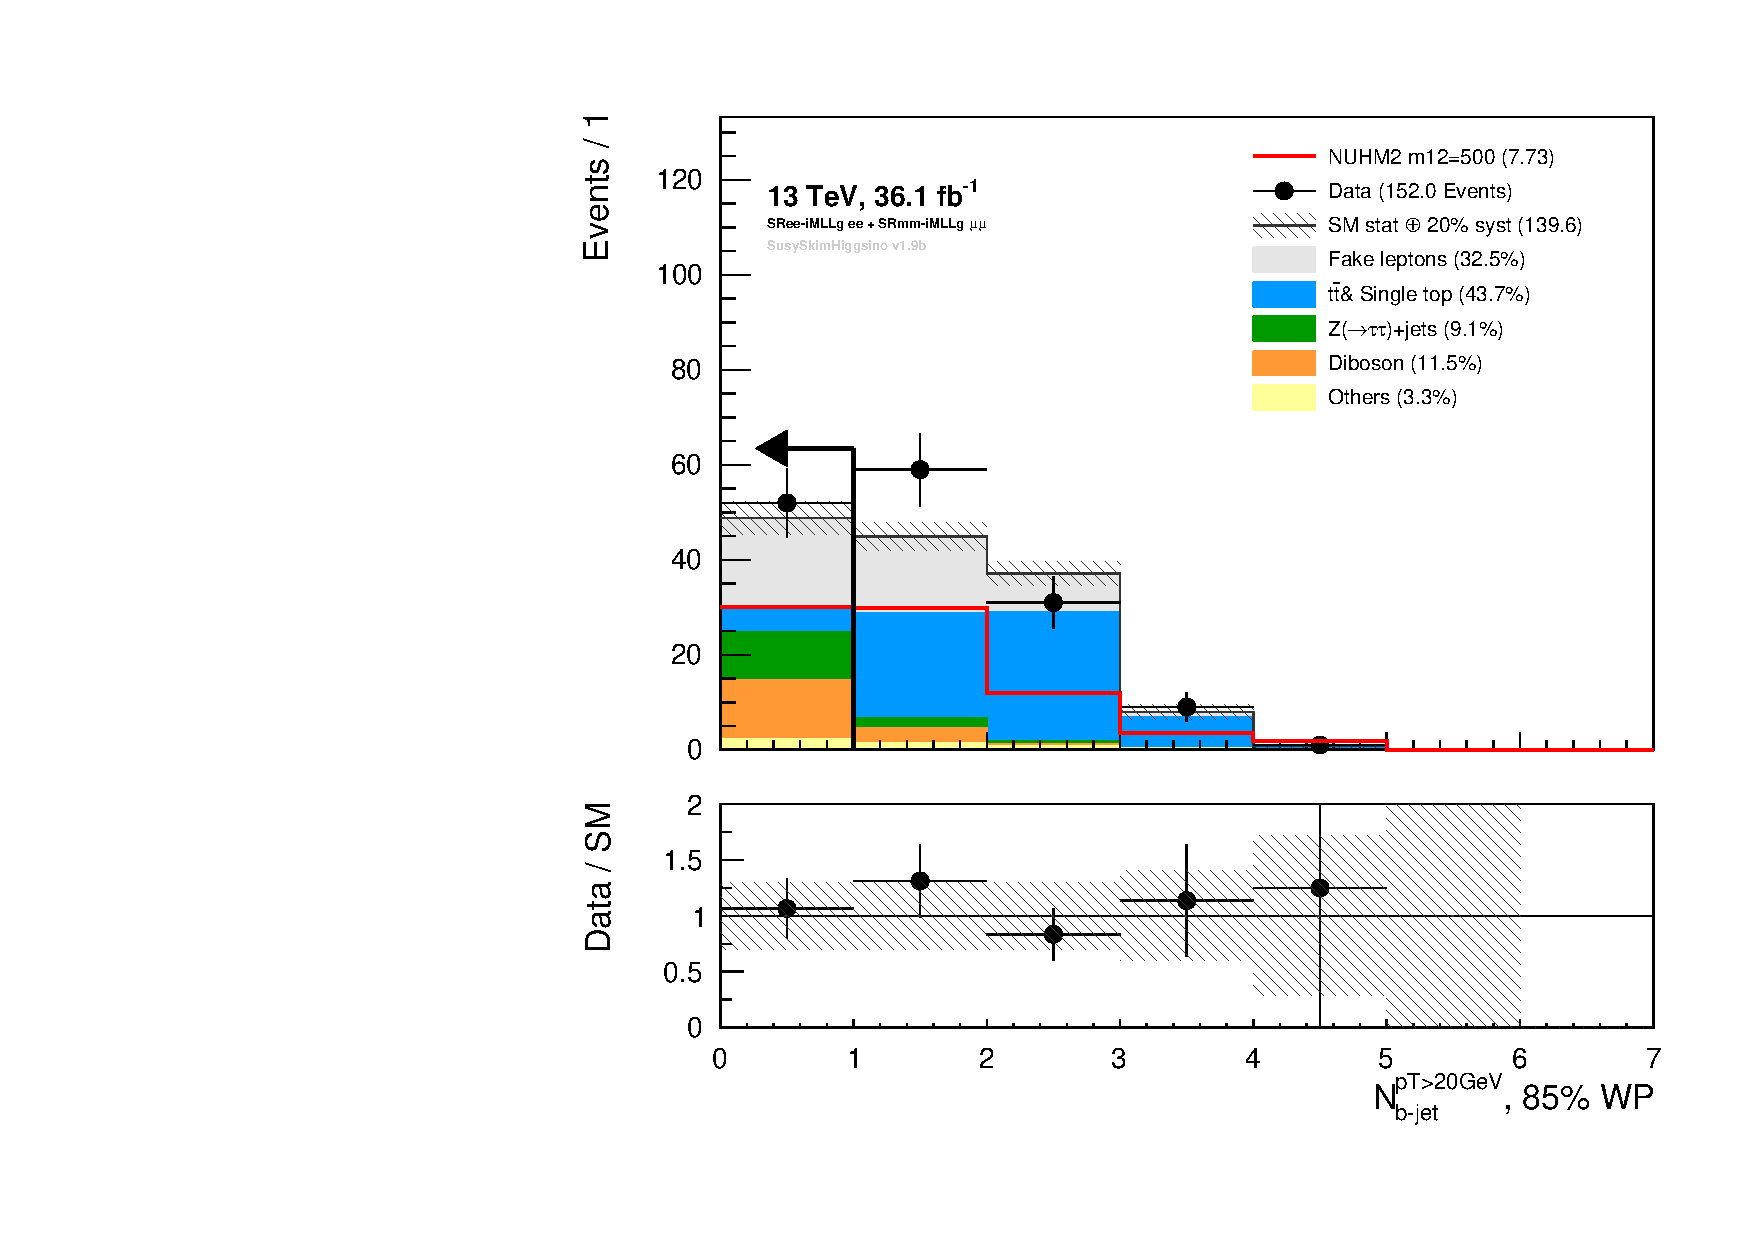
\includegraphics[scale=0.4]{NUHM2_m12_500_and_Bkg_nBJet20_MV2c10_SFOS_N_minus_one_distribution_in_SR_times_10_on_Nsig.pdf}
            \caption{$N^{20}_{\mathrm{b-jets}}$}
            \label{fig:event_nuhm2_m12_500_nBJet20_SFOS}
        \end{subfigure}
        \begin{subfigure}[b]{0.48\textwidth}
            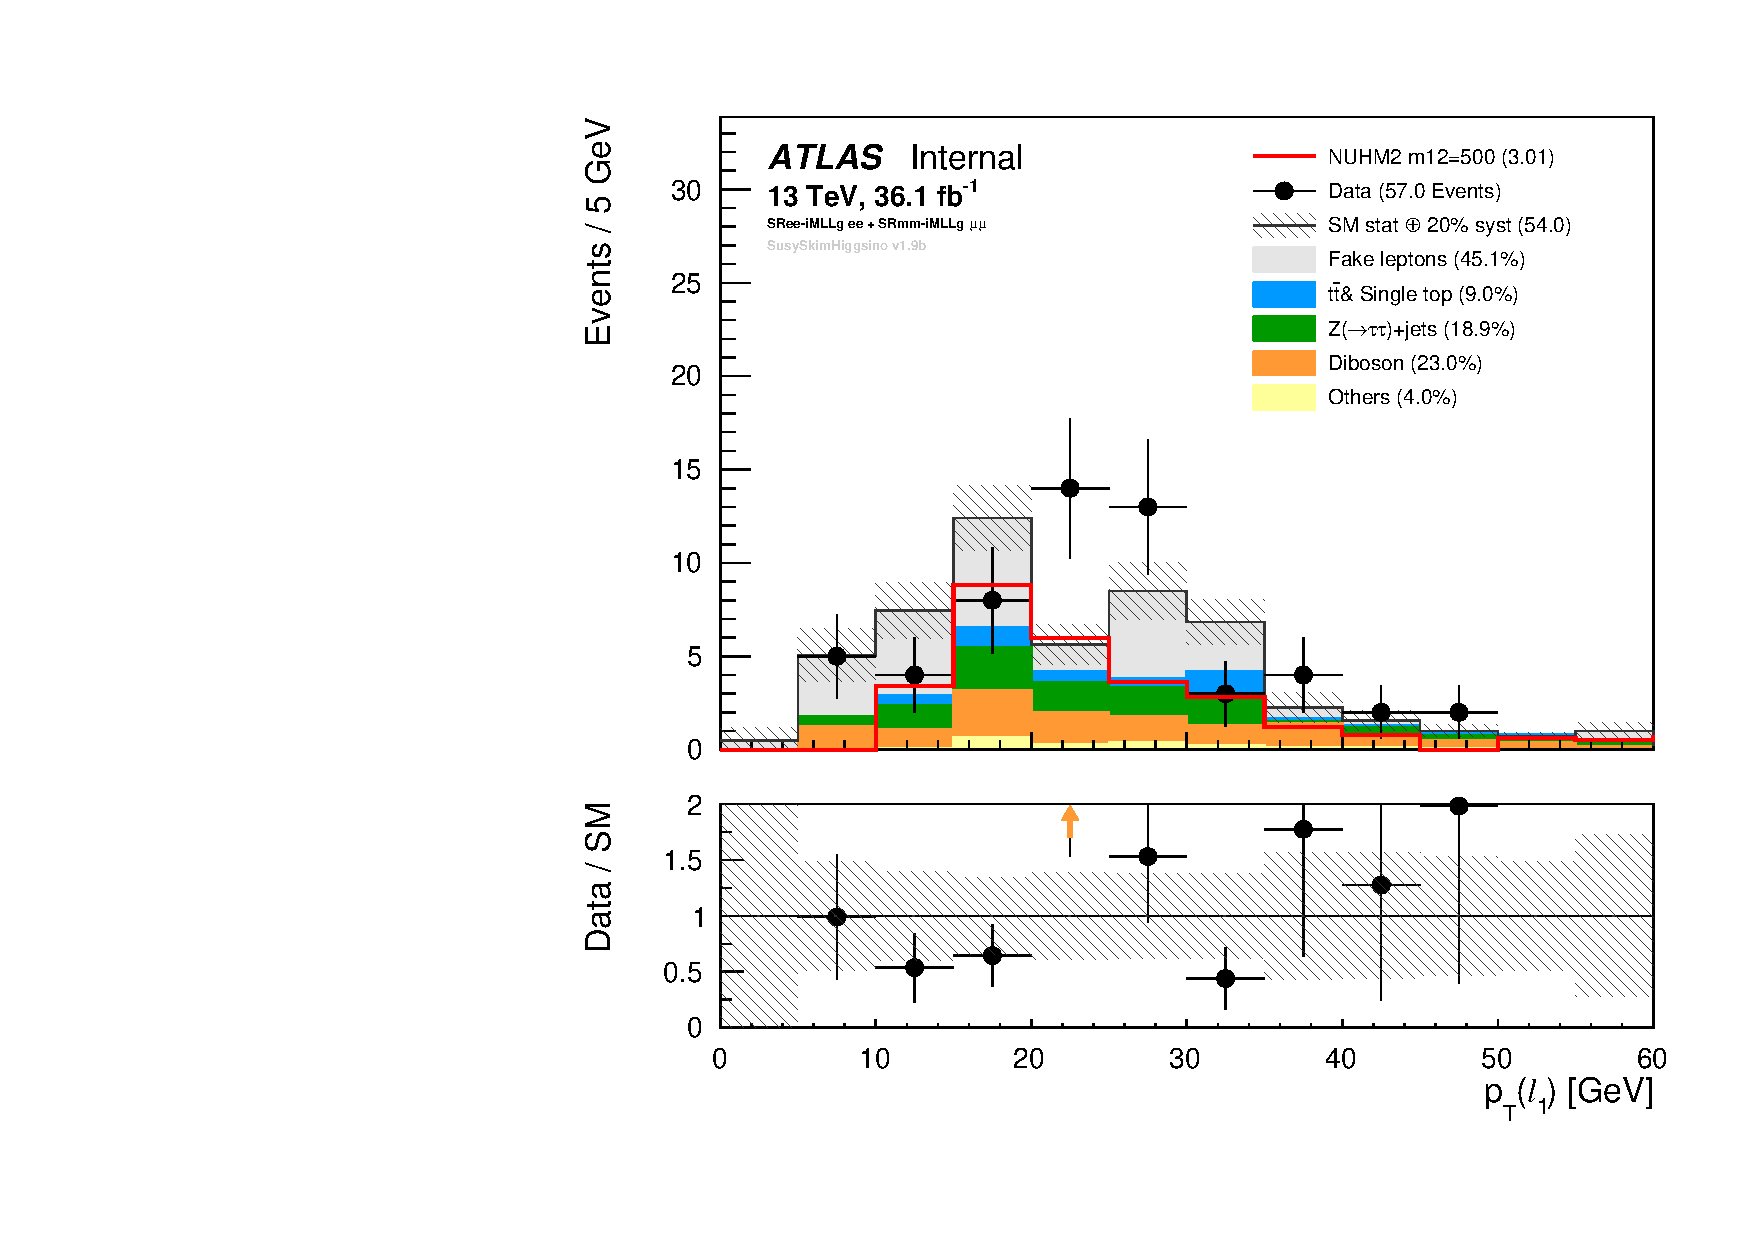
\includegraphics[scale=0.4]{NUHM2_m12_500_and_Bkg_lep1Pt_SFOS_N_minus_one_distribution_in_SR_times_10_on_Nsig.pdf}
            \caption{$p^{\ell_1}_{\mathrm{T}}$}
            \label{fig:event_nuhm2_m12_500_lep1Pt_SFOS}
        \end{subfigure}
        \begin{subfigure}[b]{0.48\textwidth}
            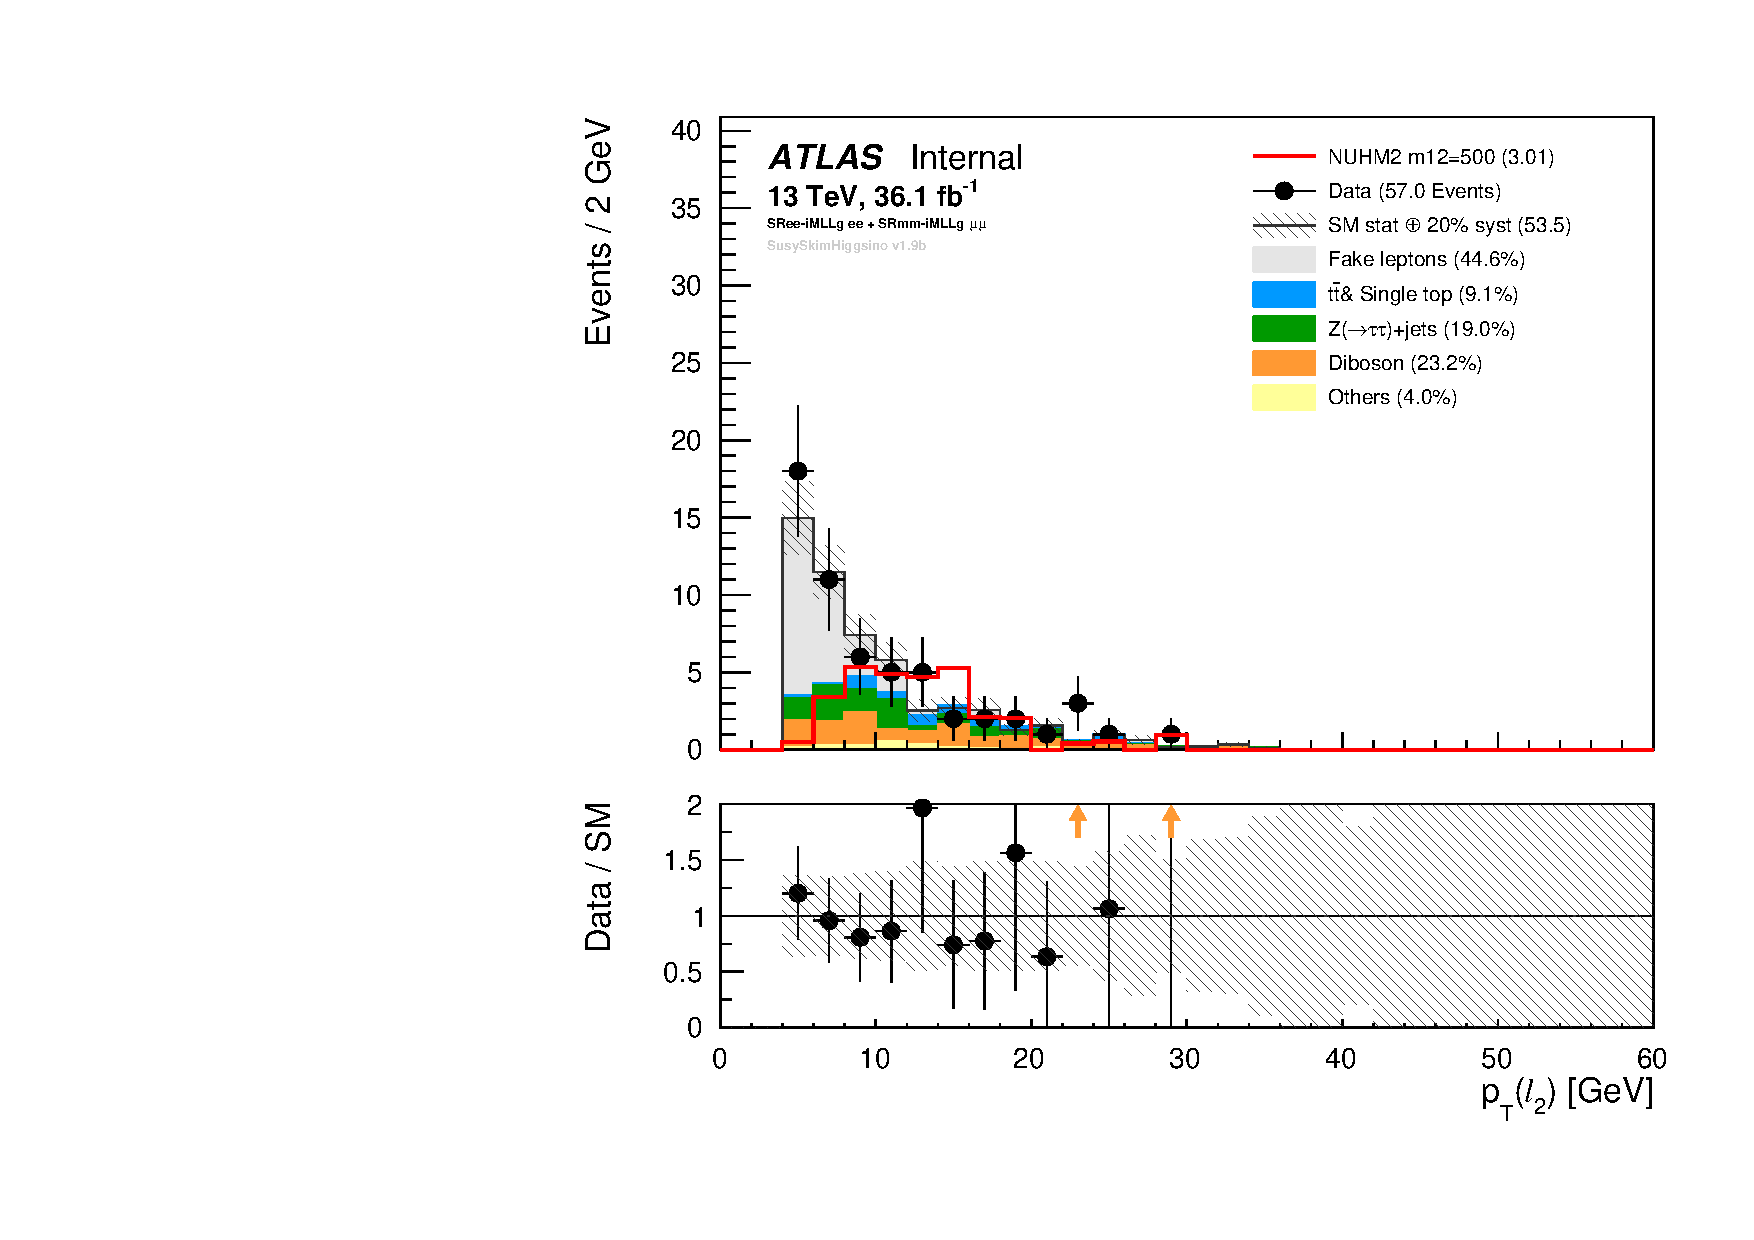
\includegraphics[scale=0.4]{NUHM2_m12_500_and_Bkg_lep2Pt_SFOS_N_minus_one_distribution_in_SR_times_10_on_Nsig.pdf}
            \caption{$p^{\ell_2}_{\mathrm{T}}$}
            \label{fig:event_nuhm2_m12_500_lep2Pt_SFOS}
        \end{subfigure}
        %\begin{subfigure}[b]{0.48\textwidth}
        %    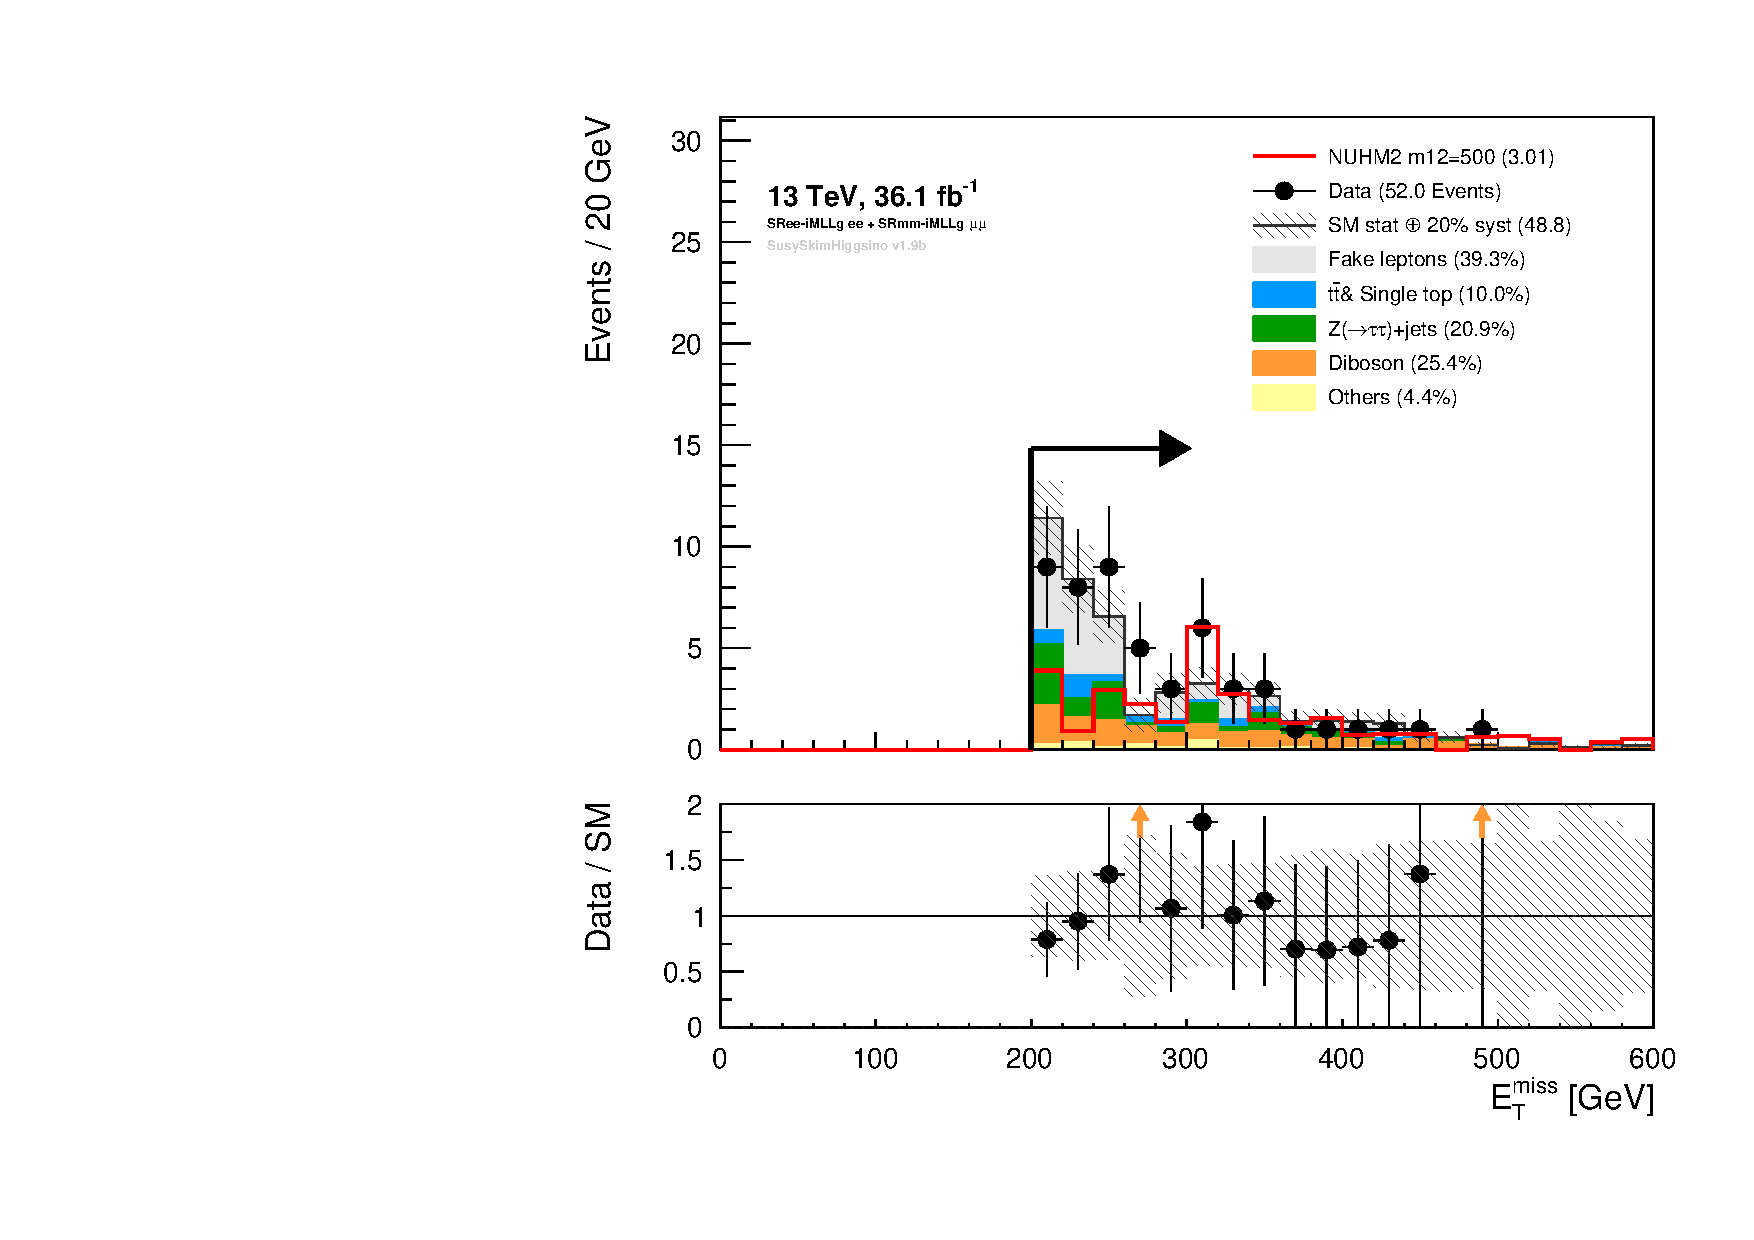
\includegraphics[scale=0.3]{NUHM2_m12_500_and_Bkg_met_Et_SFOS_N_minus_one_distribution_in_SR_times_10_on_Nsig.pdf}
        %    \caption{$E^{\mathrm{miss}}_{\mathrm{T}}$}
        %    \label{fig:event_nuhm2_m12_500_met_SFOS}
        %\end{subfigure}
        %\begin{subfigure}[b]{0.48\textwidth}
        %    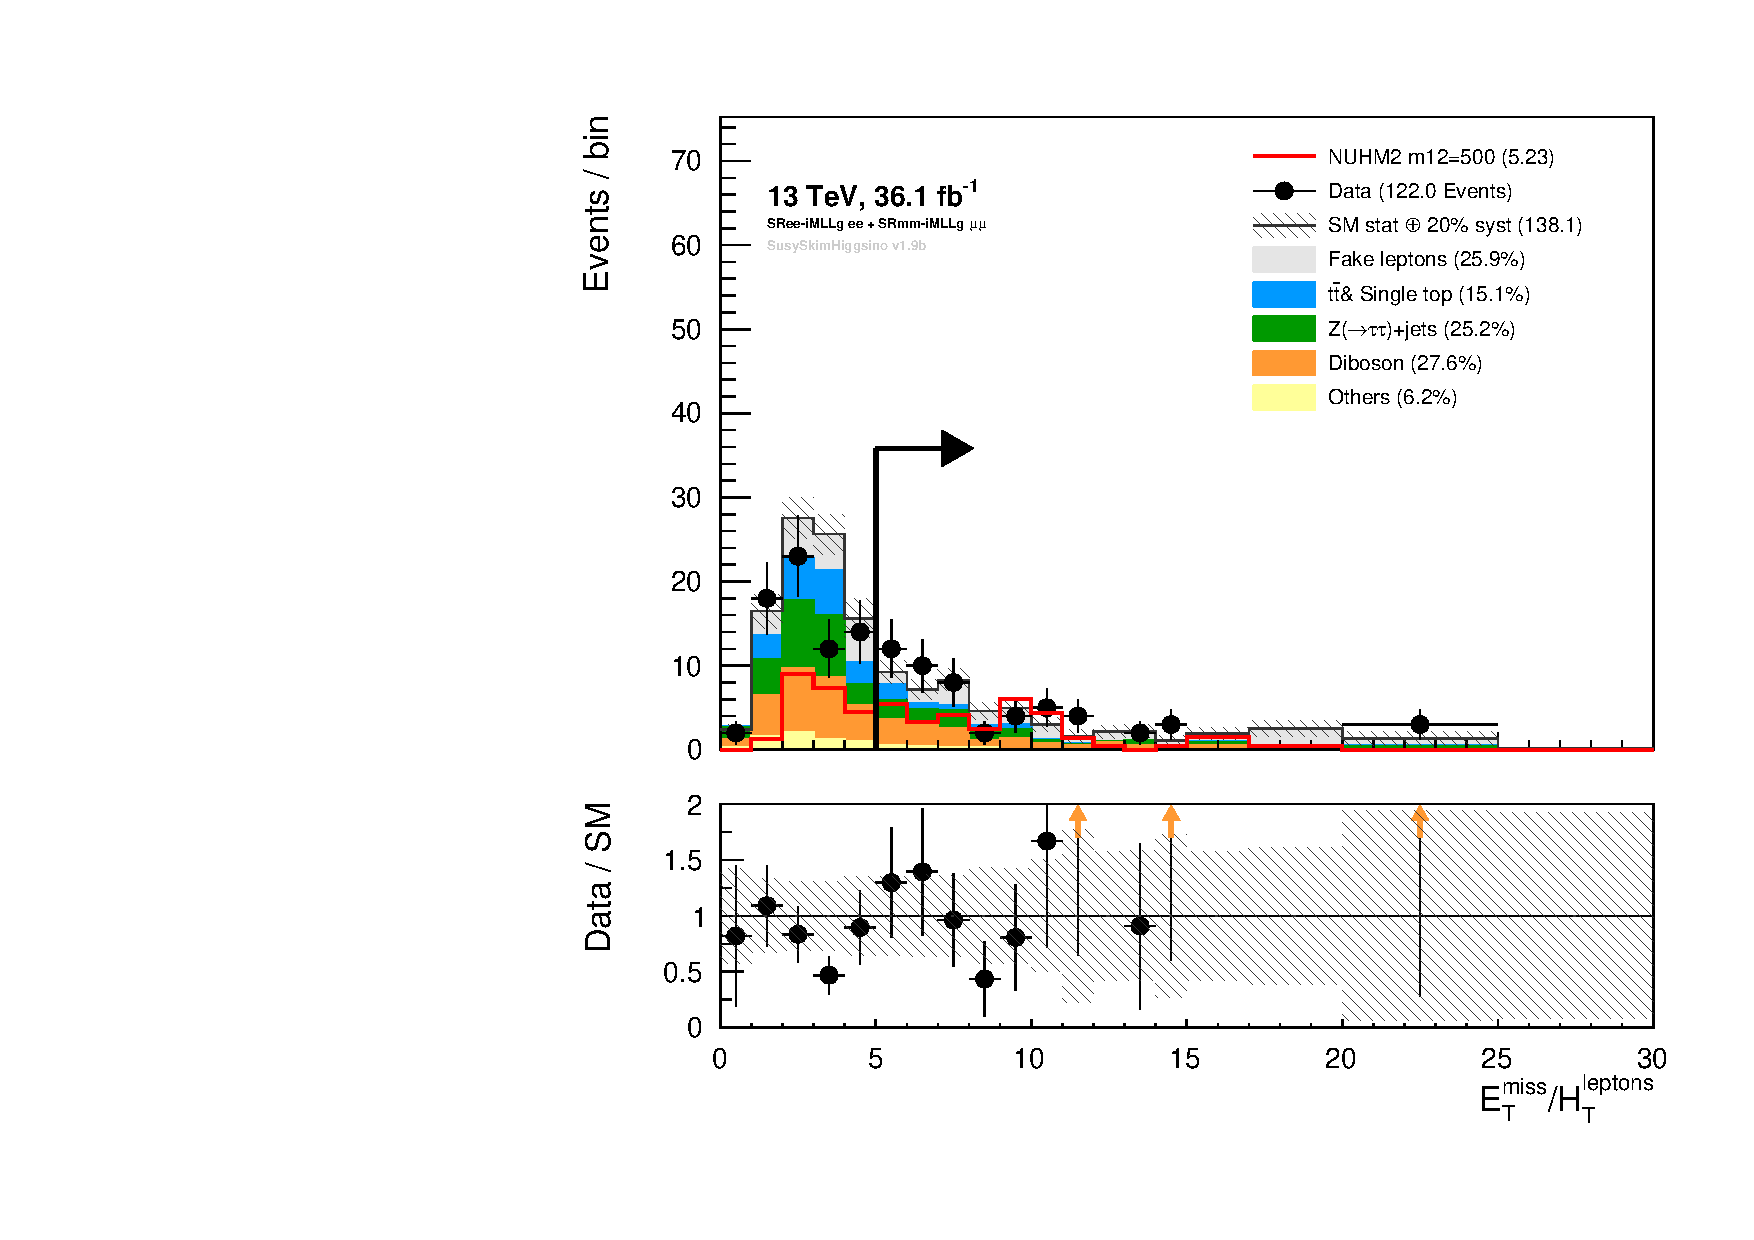
\includegraphics[scale=0.3]{NUHM2_m12_500_and_Bkg_METOverHTLep_SFOS_N_minus_one_distribution_in_SR_times_10_on_Nsig.pdf}
        %    \caption{$E^{\mathrm{miss}}_{\mathrm{T}} / H^{\mathrm{leptons}}_{\mathrm{T}}$}
        %    \label{fig:event_nuhm2_m12_500_METOverHTLep_SFOS}
        %\end{subfigure}
    \end{center}
    \caption{The `$N-1$' distributions for NUHM2 model with $m_{1/2} = 500$~{\GeV} in SR region $1 < $SR$\ell \ell$-$m_{\ell \ell} < 60$~{\GeV}.
    The NUHM2 distributions are multiplied by 10 but the number of events in the legend use its actual values.
    %The distributions of $N_\mathrm{jets}^{30}$, $N_\mathrm{b-jets}^{20}$, $\pt^{\ell_{1}}$, $\pt^{\ell_{2}}$, \met, and $\met/H_\mathrm{T}^\mathrm{leptons}$ are shown.}
    The distributions of $N_\mathrm{jets}^{30}$, $N_\mathrm{b-jets}^{20}$, $\pt^{\ell_{1}}$, and $\pt^{\ell_{2}}$ are shown.}
    \label{fig:event_nuhm2_kinematic_in_SR_SFOS_1}
\end{figure}

\begin{figure}[htbp]
    \begin{center}
        \begin{subfigure}[b]{0.48\textwidth}
            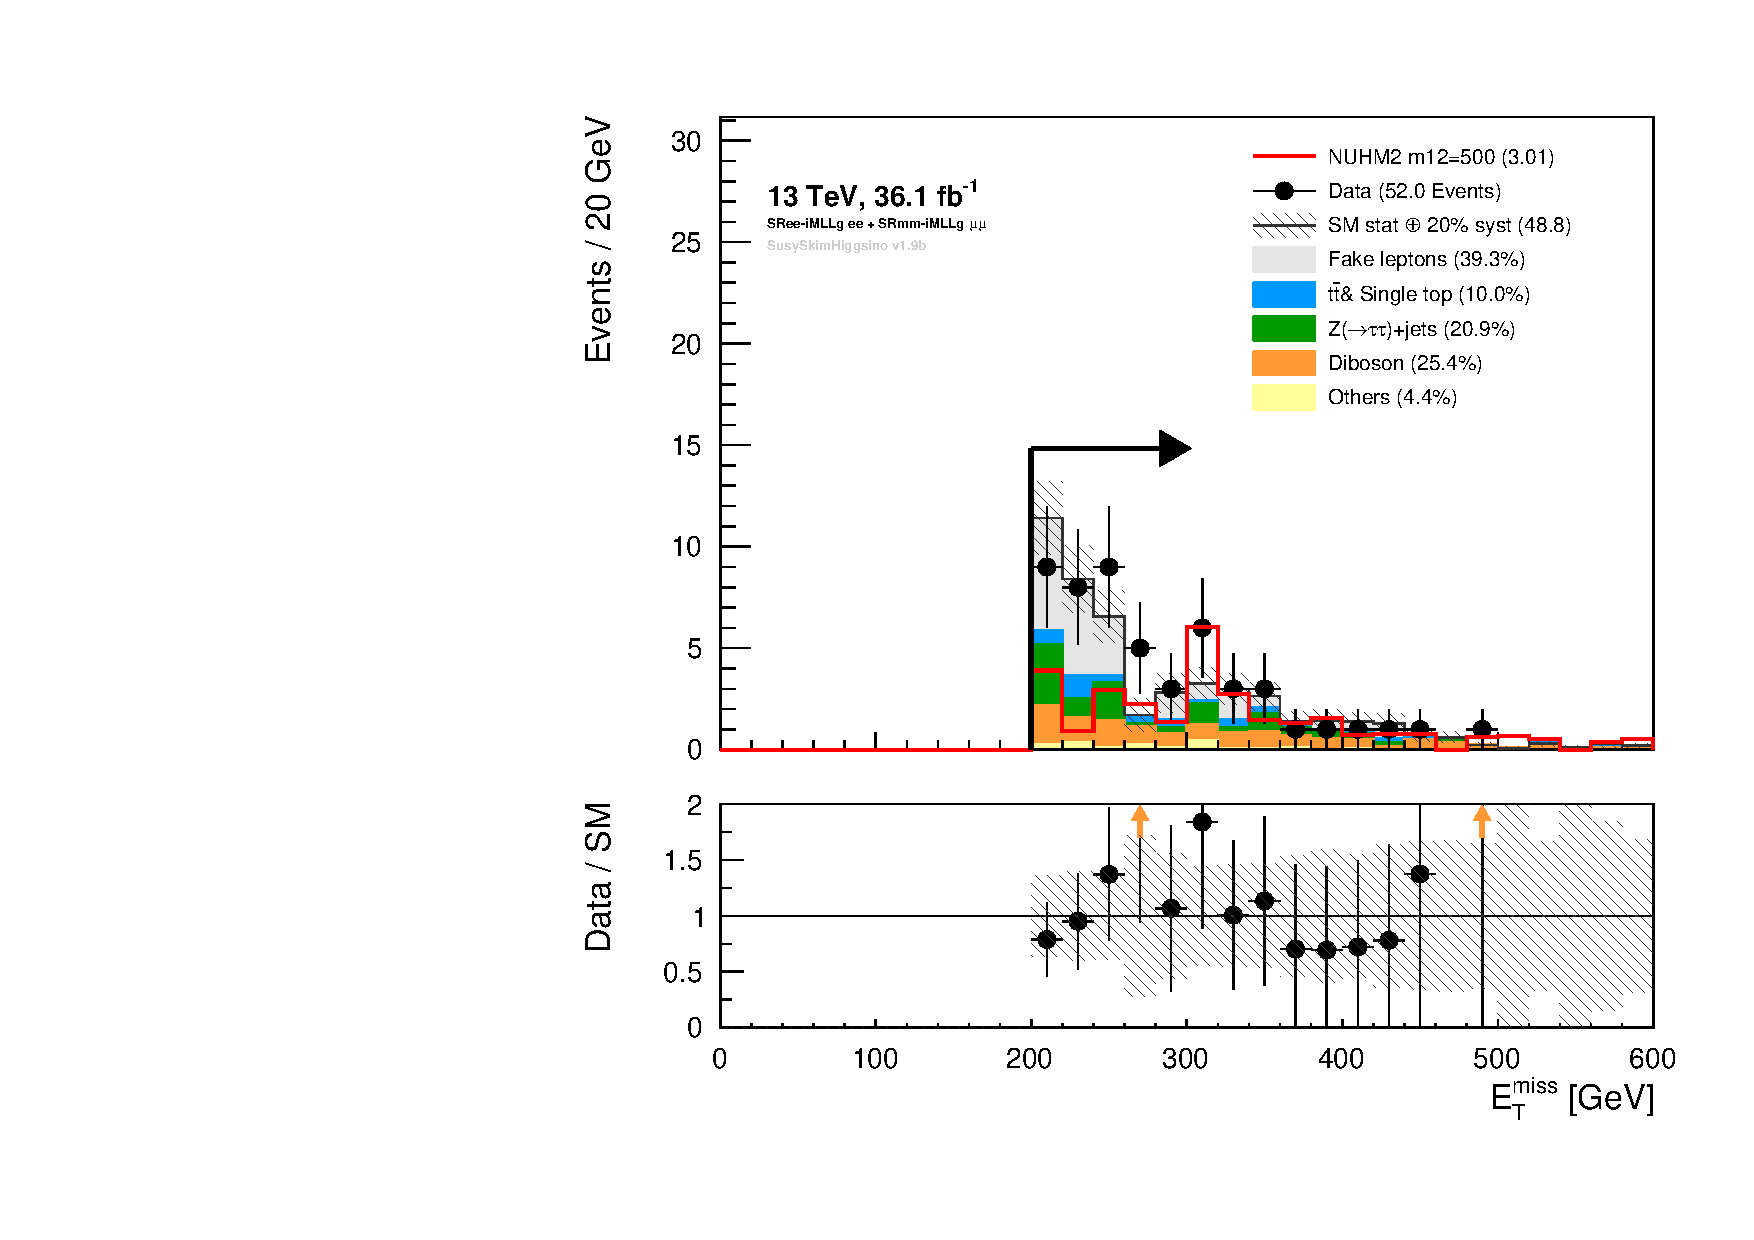
\includegraphics[scale=0.4]{NUHM2_m12_500_and_Bkg_met_Et_SFOS_N_minus_one_distribution_in_SR_times_10_on_Nsig.pdf}
            \caption{$E^{\mathrm{miss}}_{\mathrm{T}}$}
            \label{fig:event_nuhm2_m12_500_met_SFOS}
        \end{subfigure}
        \begin{subfigure}[b]{0.48\textwidth}
            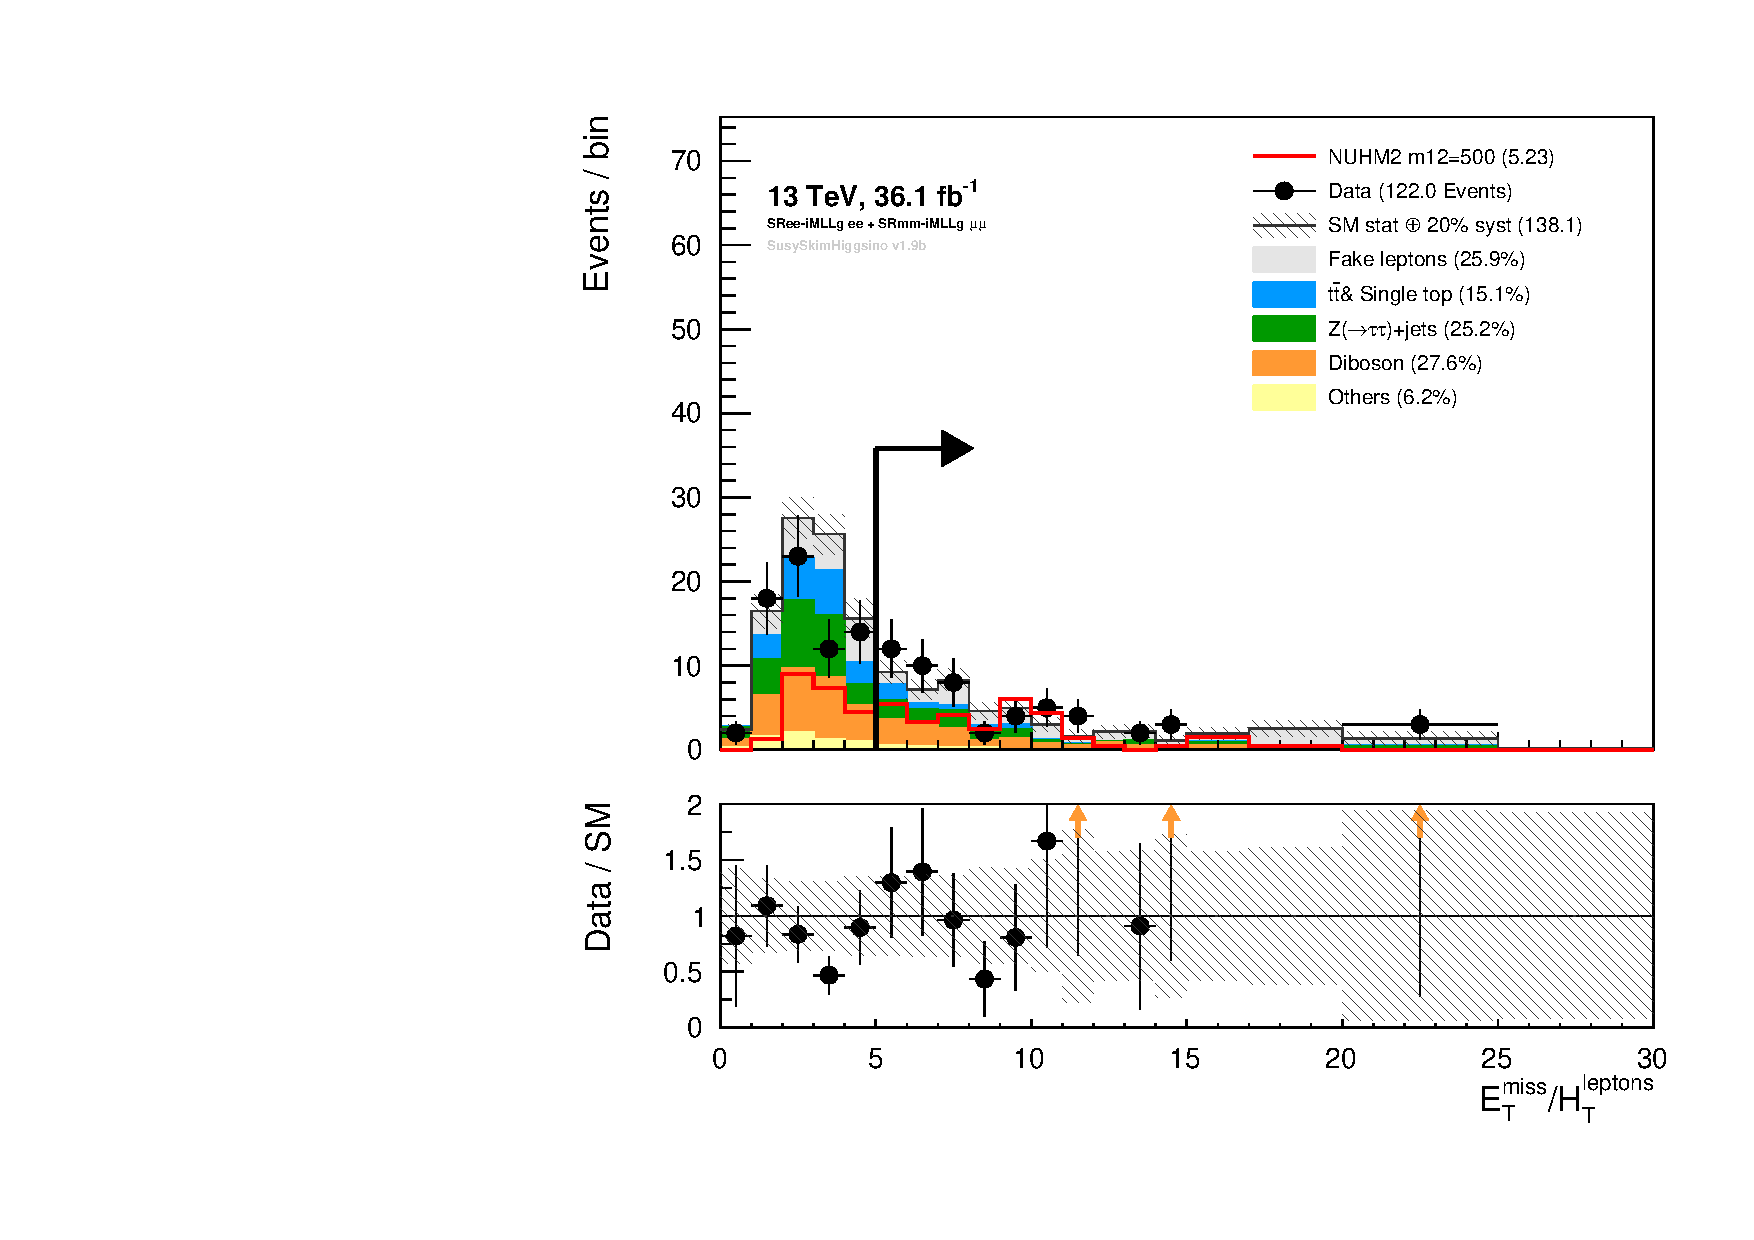
\includegraphics[scale=0.4]{NUHM2_m12_500_and_Bkg_METOverHTLep_SFOS_N_minus_one_distribution_in_SR_times_10_on_Nsig.pdf}
            \caption{$E^{\mathrm{miss}}_{\mathrm{T}} / H^{\mathrm{leptons}}_{\mathrm{T}}$}
            \label{fig:event_nuhm2_m12_500_METOverHTLep_SFOS}
        \end{subfigure}
        \begin{subfigure}[b]{0.48\textwidth}
            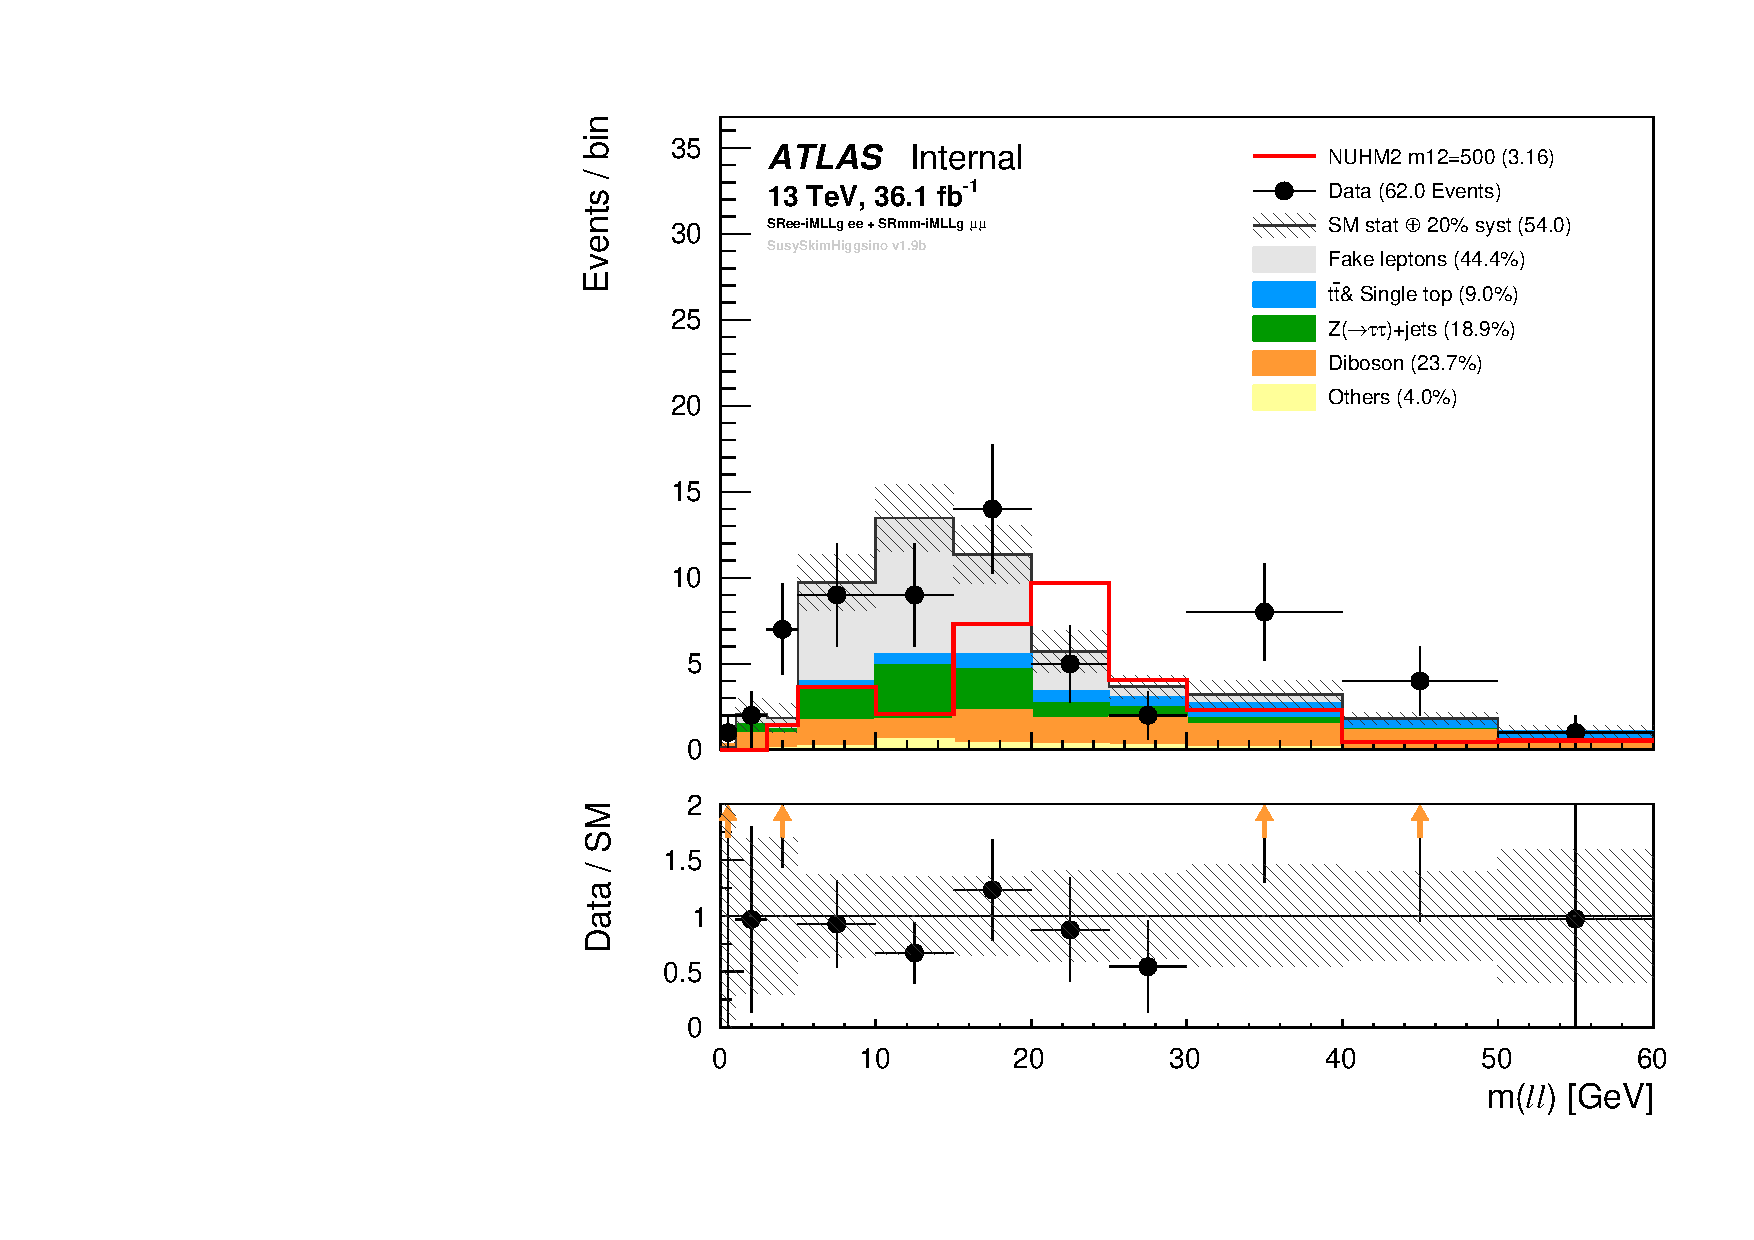
\includegraphics[scale=0.4]{NUHM2_m12_500_and_Bkg_mll_SFOS_N_minus_one_distribution_in_SR_times_10_on_Nsig.pdf}
            \caption{$m_{\ell\ell}$}
            \label{fig:event_nuhm2_m12_500_mll_SFOS}
        \end{subfigure}
        \begin{subfigure}[b]{0.48\textwidth}
            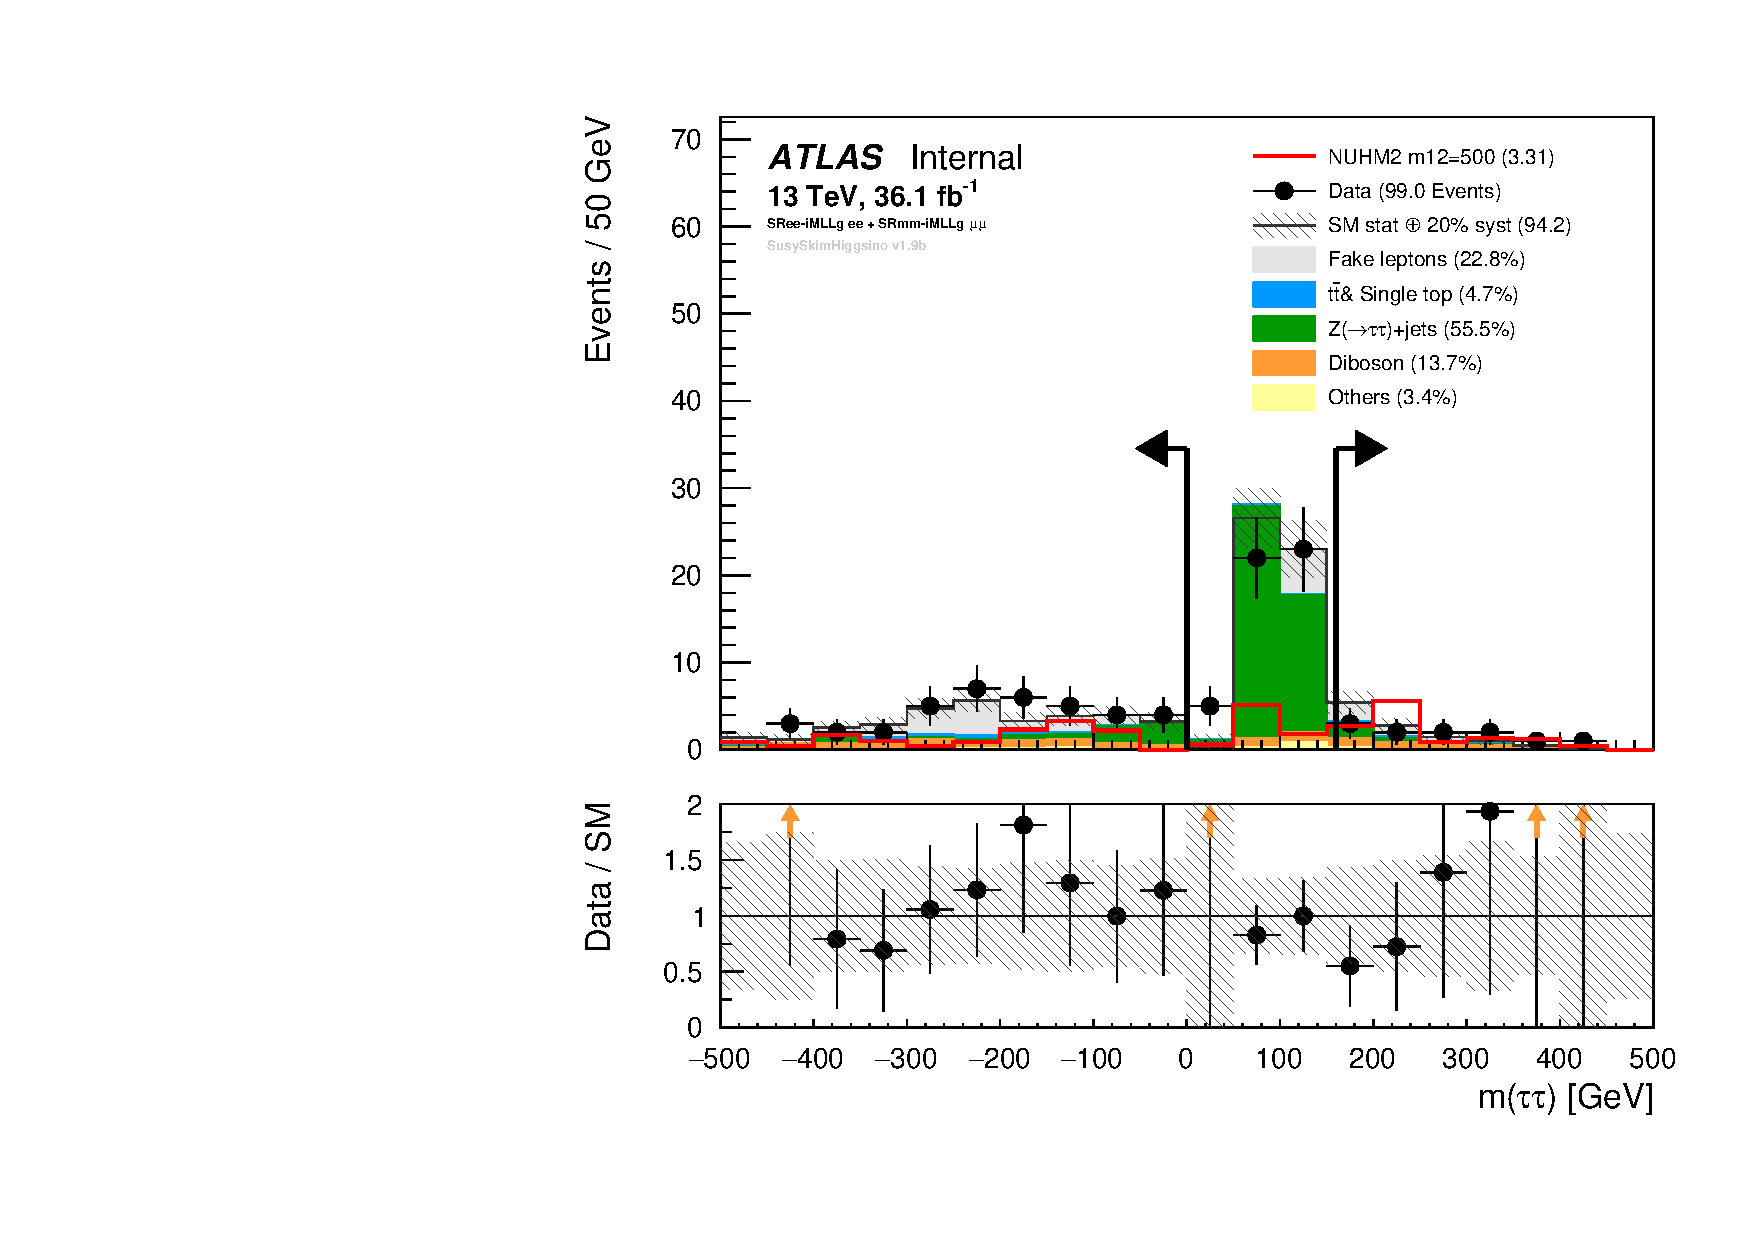
\includegraphics[scale=0.4]{NUHM2_m12_500_and_Bkg_MTauTau_SFOS_N_minus_one_distribution_in_SR_times_10_on_Nsig.pdf}
            \caption{$m_{\tau\tau}$}
            \label{fig:event_nuhm2_m12_500_MTauTau_SFOS}
        \end{subfigure}
    \end{center}
    \caption{The `$N-1$' distributions for NUHM2 model with $m_{1/2} = 500$~{\GeV} in SR region $1 < $SR$\ell \ell$-$m_{\ell \ell} < 60$~{\GeV}.
    The NUHM2 distributions are multiplied by 10 but the number of events in the legend use its actual values.
    The distributions of \met, $\met/H_\mathrm{T}^\mathrm{leptons}$, $m_{\ell \ell}$, and $m_{\tau \tau}$ are shown.}
    \label{fig:event_nuhm2_kinematic_in_SR_SFOS_2}
\end{figure}

\begin{figure}[htbp]
    \begin{center}
        %\begin{subfigure}[b]{0.48\textwidth}
        %    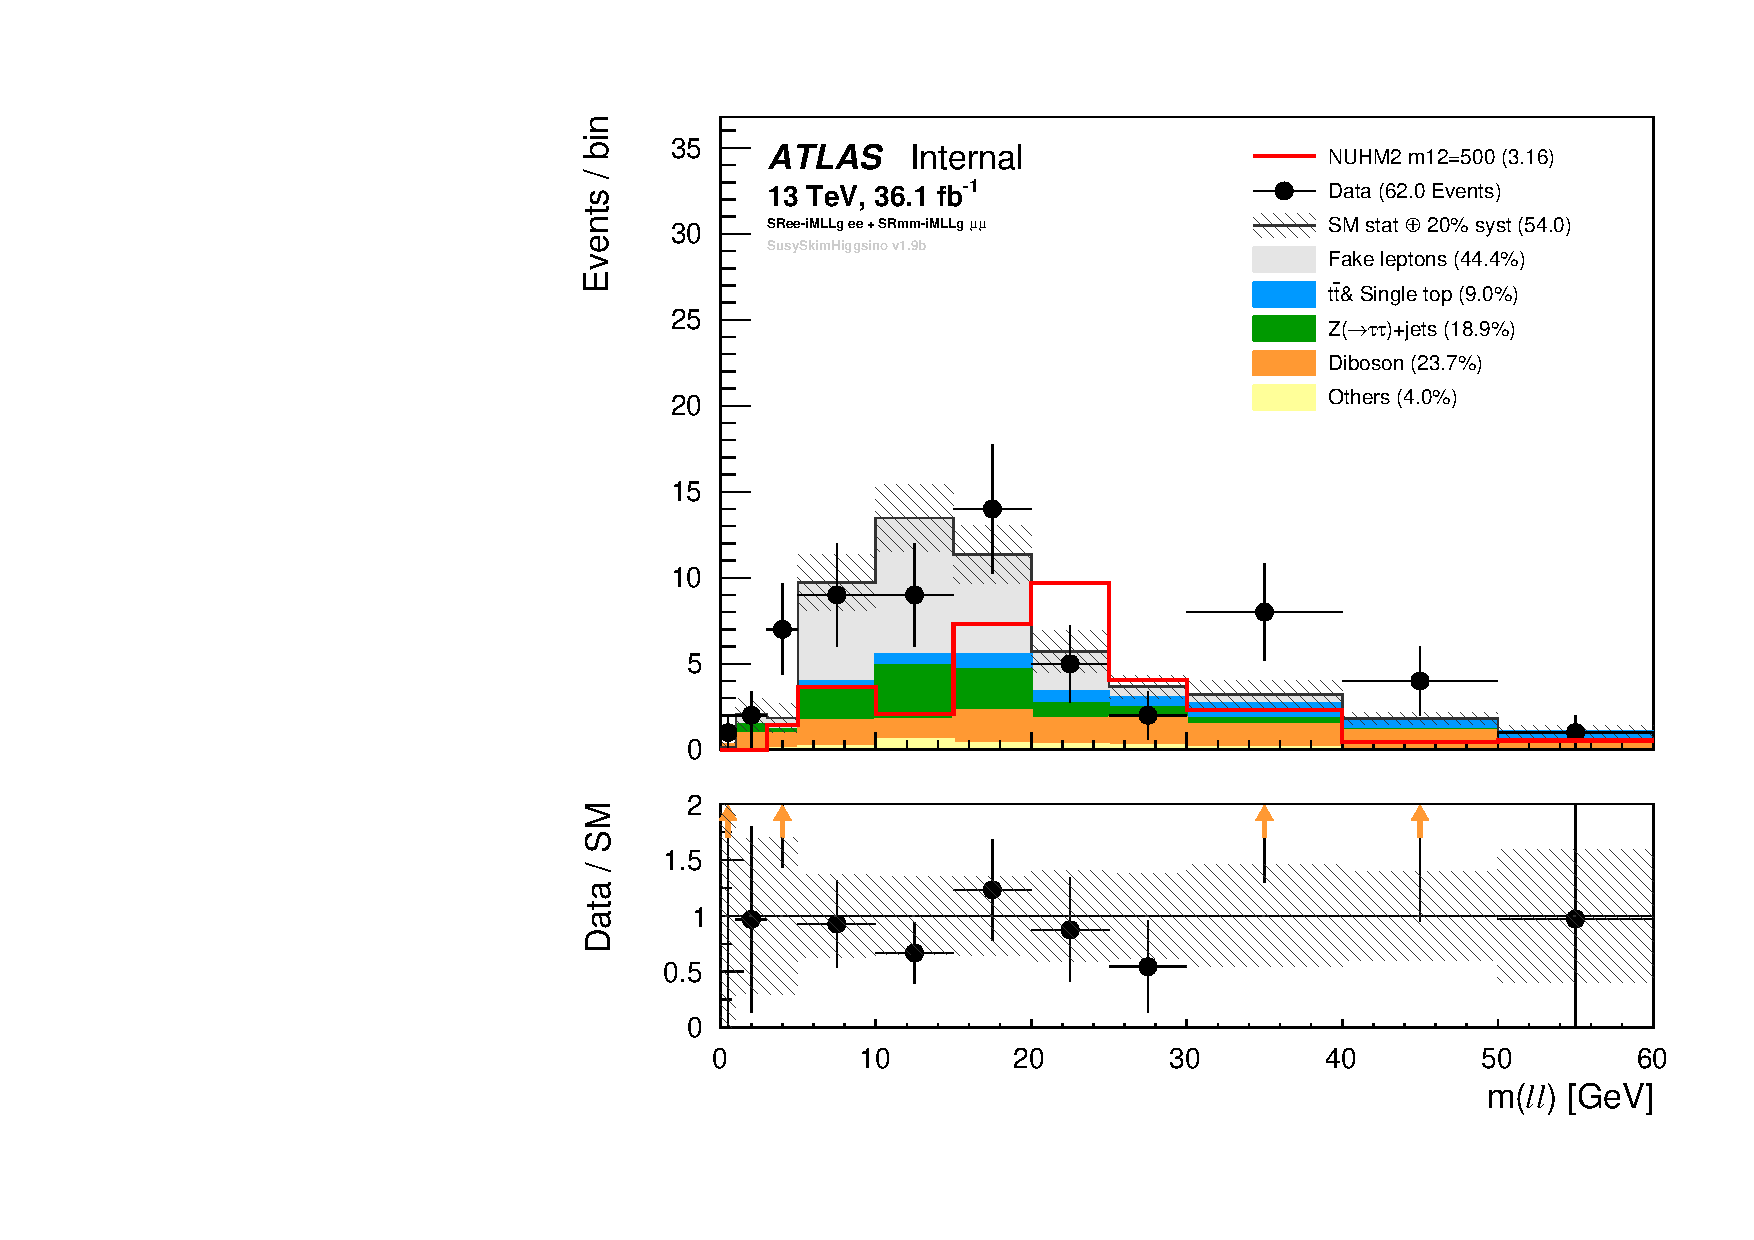
\includegraphics[scale=0.3]{NUHM2_m12_500_and_Bkg_mll_SFOS_N_minus_one_distribution_in_SR_times_10_on_Nsig.pdf}
        %    \caption{$m_{\ell\ell}$}
        %    \label{fig:event_nuhm2_m12_500_mll_SFOS}
        %\end{subfigure}
        %\begin{subfigure}[b]{0.48\textwidth}
        %    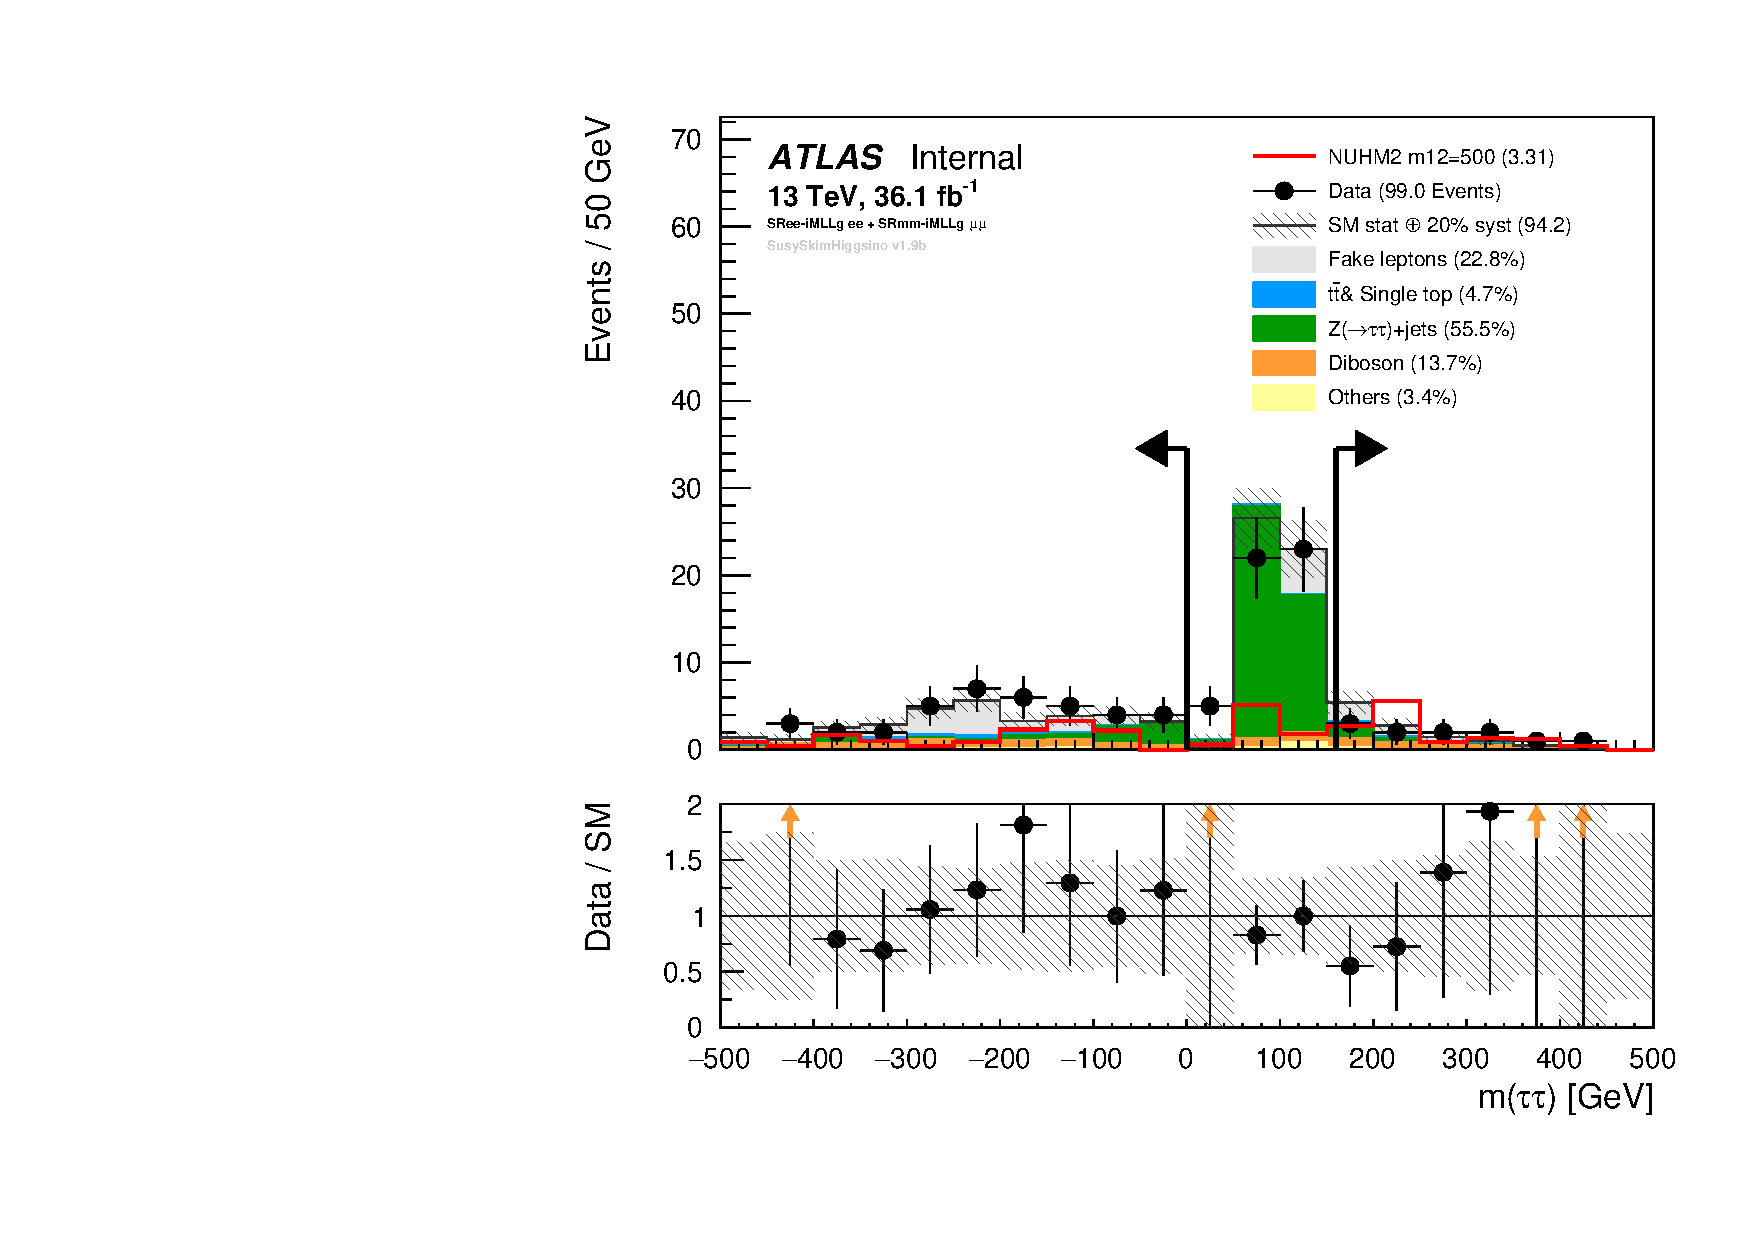
\includegraphics[scale=0.3]{NUHM2_m12_500_and_Bkg_MTauTau_SFOS_N_minus_one_distribution_in_SR_times_10_on_Nsig.pdf}
        %    \caption{$m_{\tau\tau}$}
        %    \label{fig:event_nuhm2_m12_500_MTauTau_SFOS}
        %\end{subfigure}
        \begin{subfigure}[b]{0.48\textwidth}
            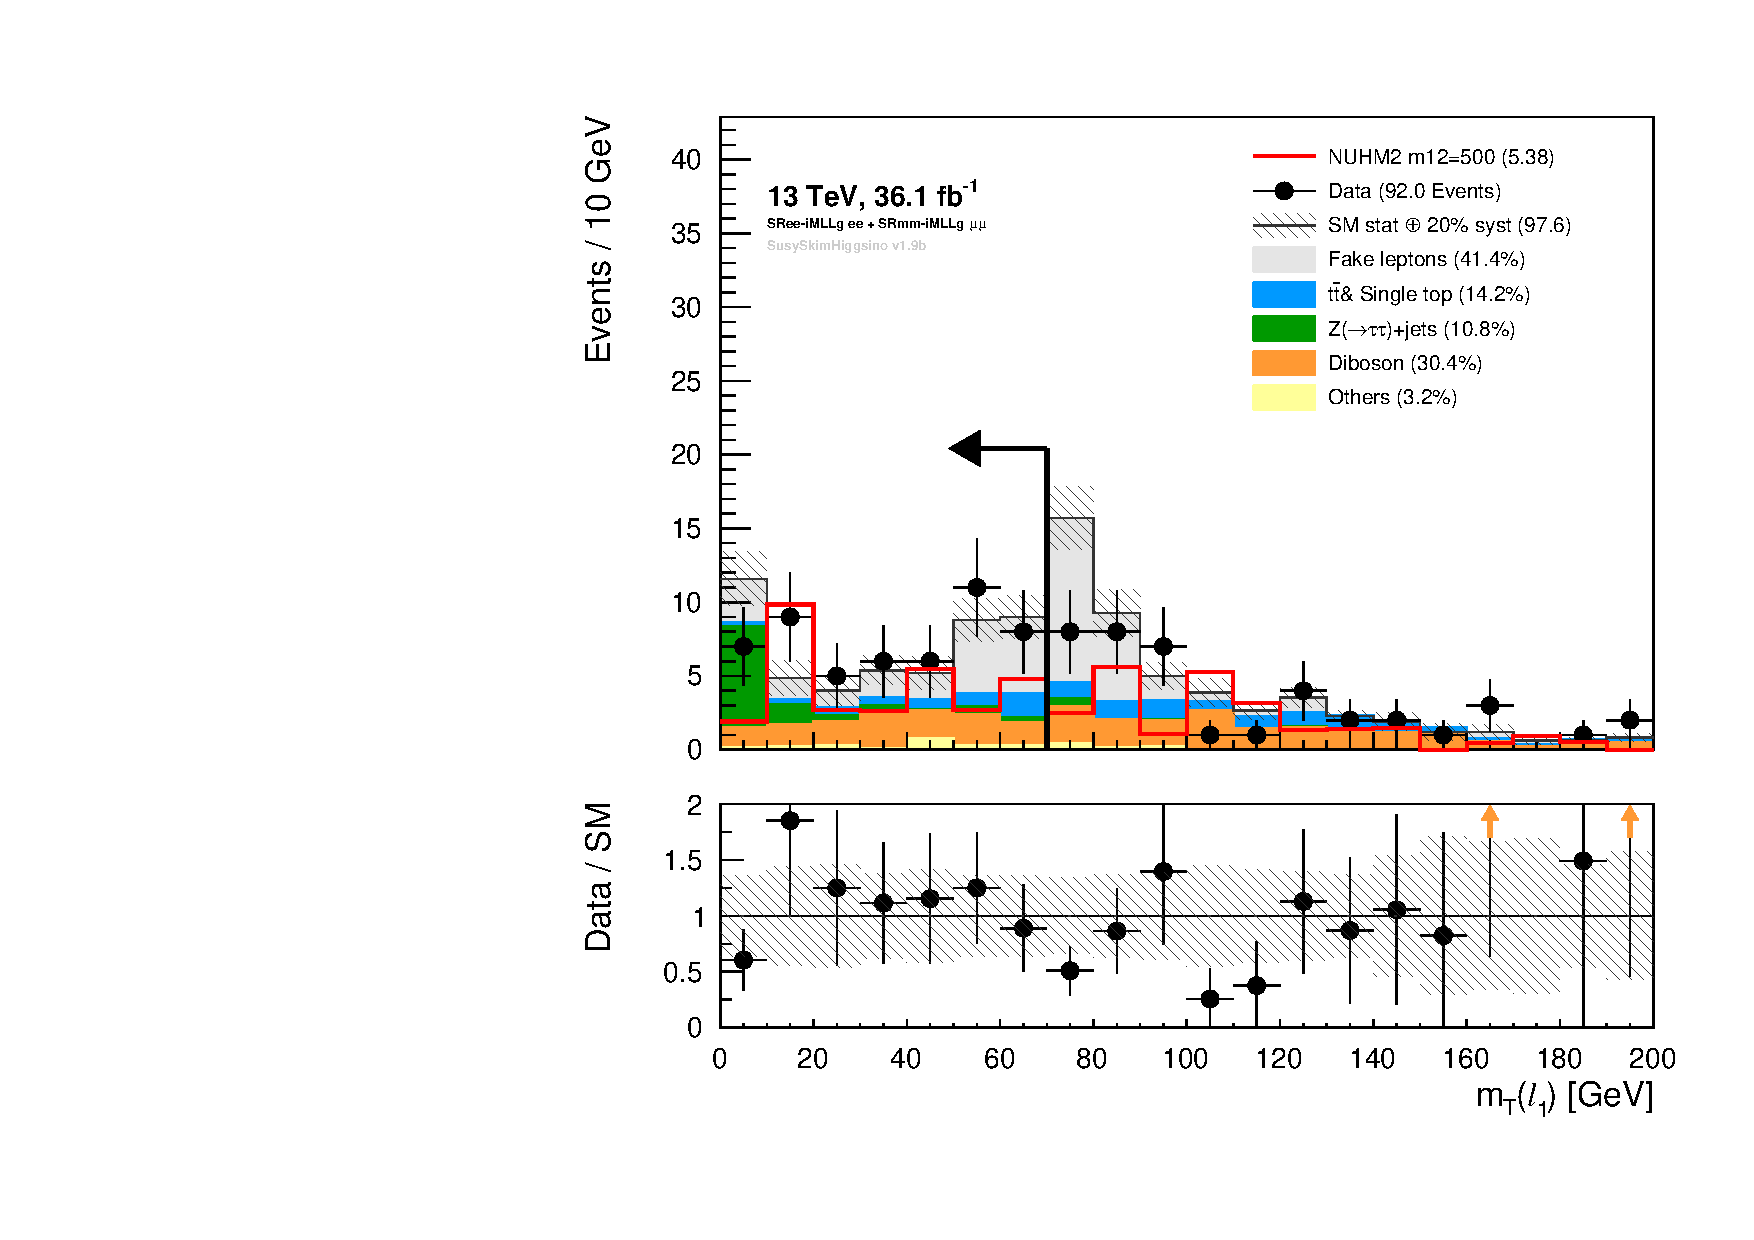
\includegraphics[scale=0.4]{NUHM2_m12_500_and_Bkg_mt_lep1_SFOS_N_minus_one_distribution_in_SR_times_10_on_Nsig.pdf}
            \caption{$m_{T}(\ell_{1})$}
            \label{fig:event_nuhm2_m12_500_mt_lep1_SFOS}
        \end{subfigure}
        \begin{subfigure}[b]{0.48\textwidth}
            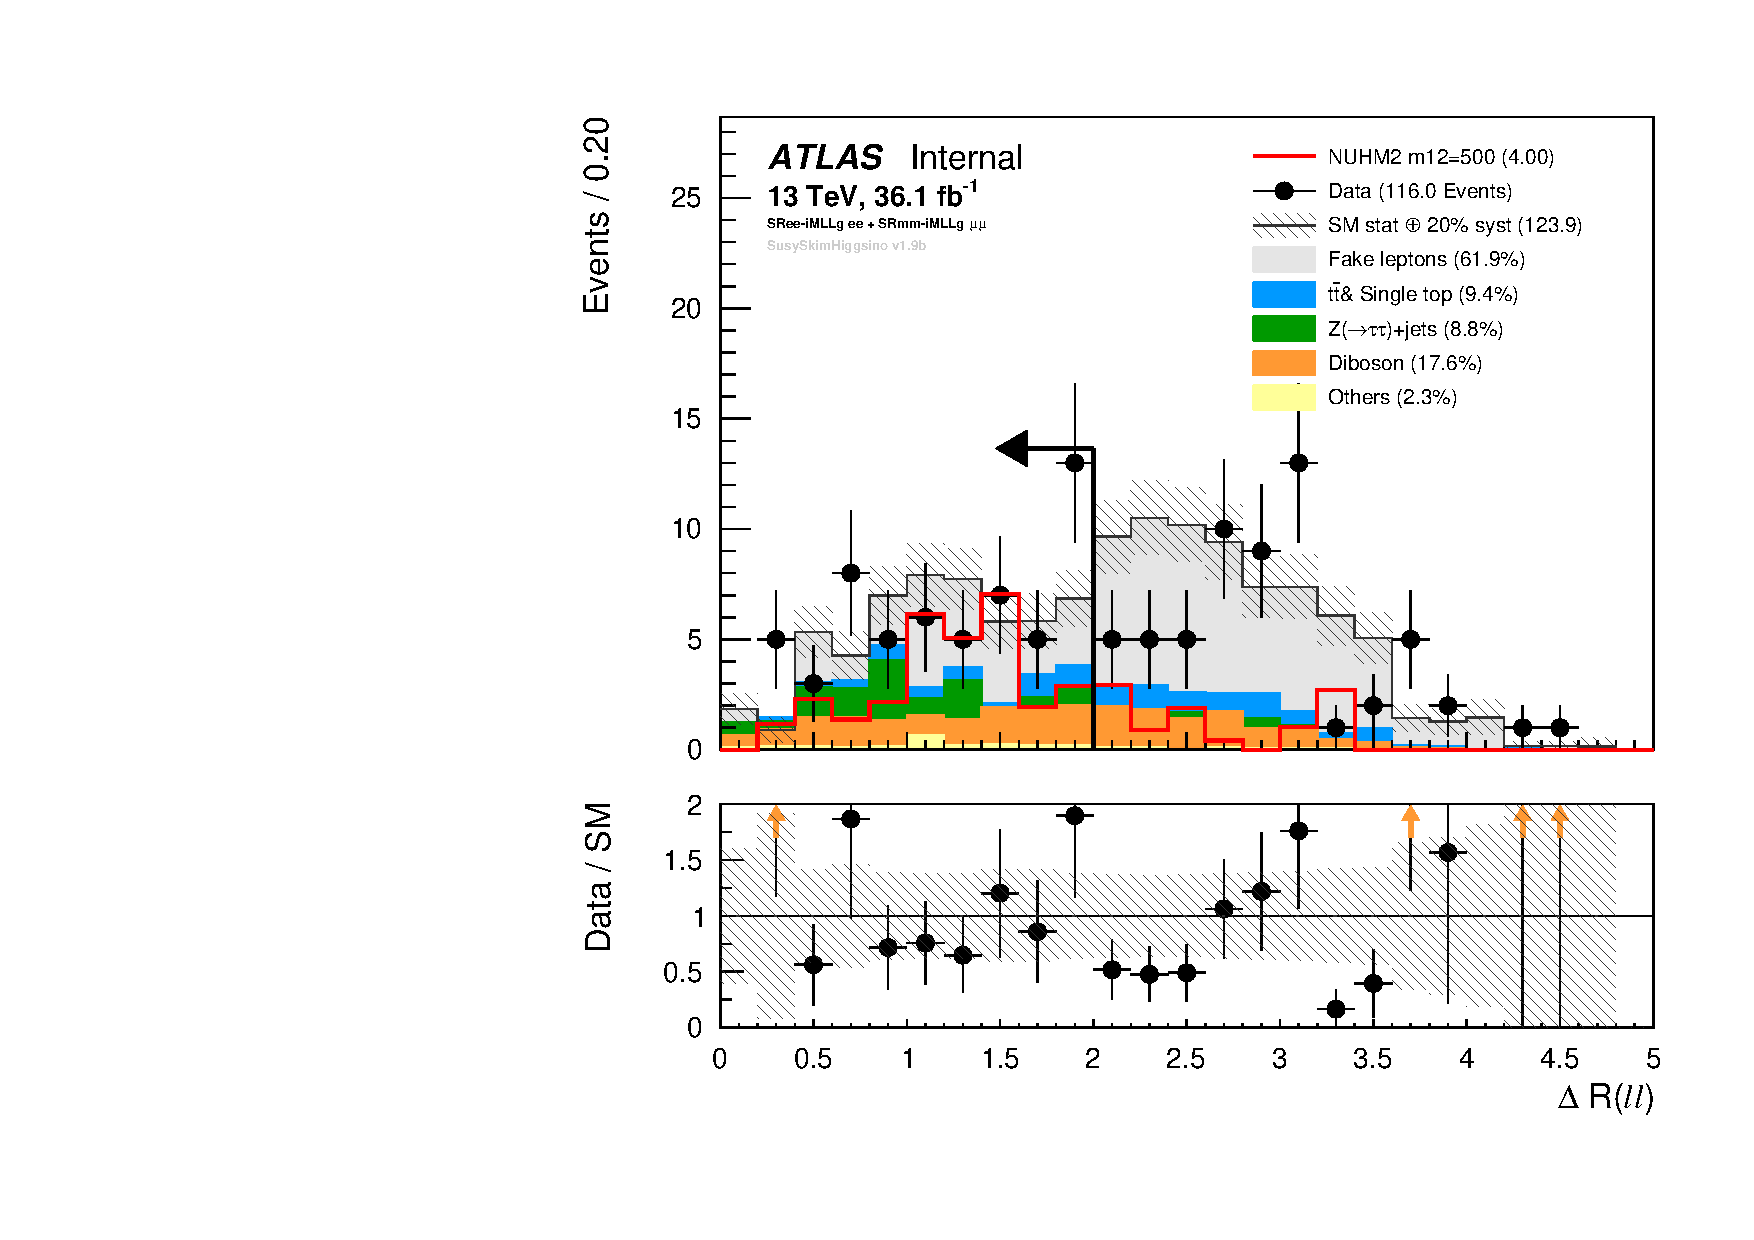
\includegraphics[scale=0.4]{NUHM2_m12_500_and_Bkg_Rll_SFOS_N_minus_one_distribution_in_SR_times_10_on_Nsig.pdf}
            \caption{$\Delta R_{\ell\ell}$}
            \label{fig:event_nuhm2_m12_500_Rll_SFOS}
        \end{subfigure}
        \begin{subfigure}[b]{0.48\textwidth}
            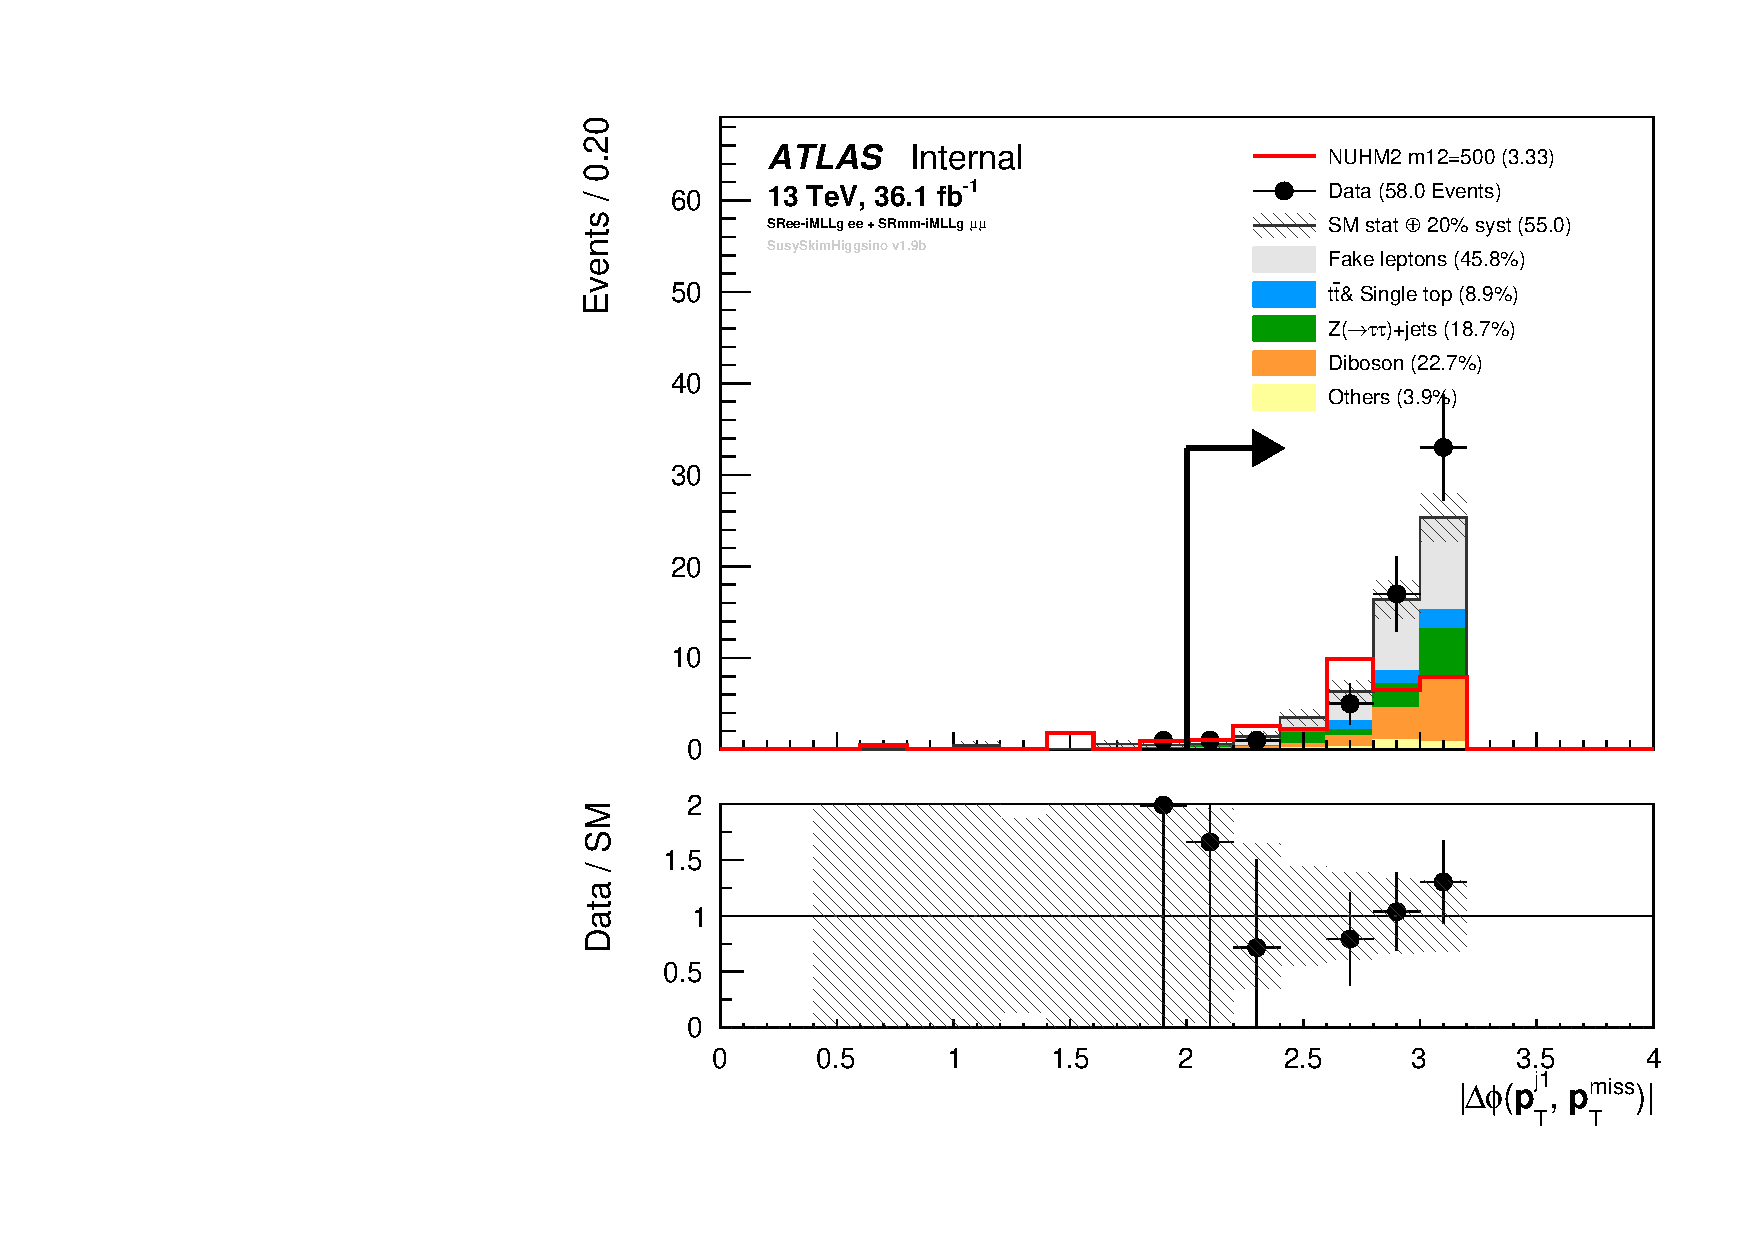
\includegraphics[scale=0.4]{NUHM2_m12_500_and_Bkg_DPhiJ1Met_SFOS_N_minus_one_distribution_in_SR_times_10_on_Nsig.pdf}
            \caption{$|\Delta \phi(\mathbf{p}^{j_{1}}_{\mathrm{T}}, \mathbf{p}^{\mathrm{miss}}_{\mathrm{T}})|$}
            \label{fig:event_nuhm2_m12_500_DPhiJ1Met_SFOS}
        \end{subfigure}
        \begin{subfigure}[b]{0.48\textwidth}
            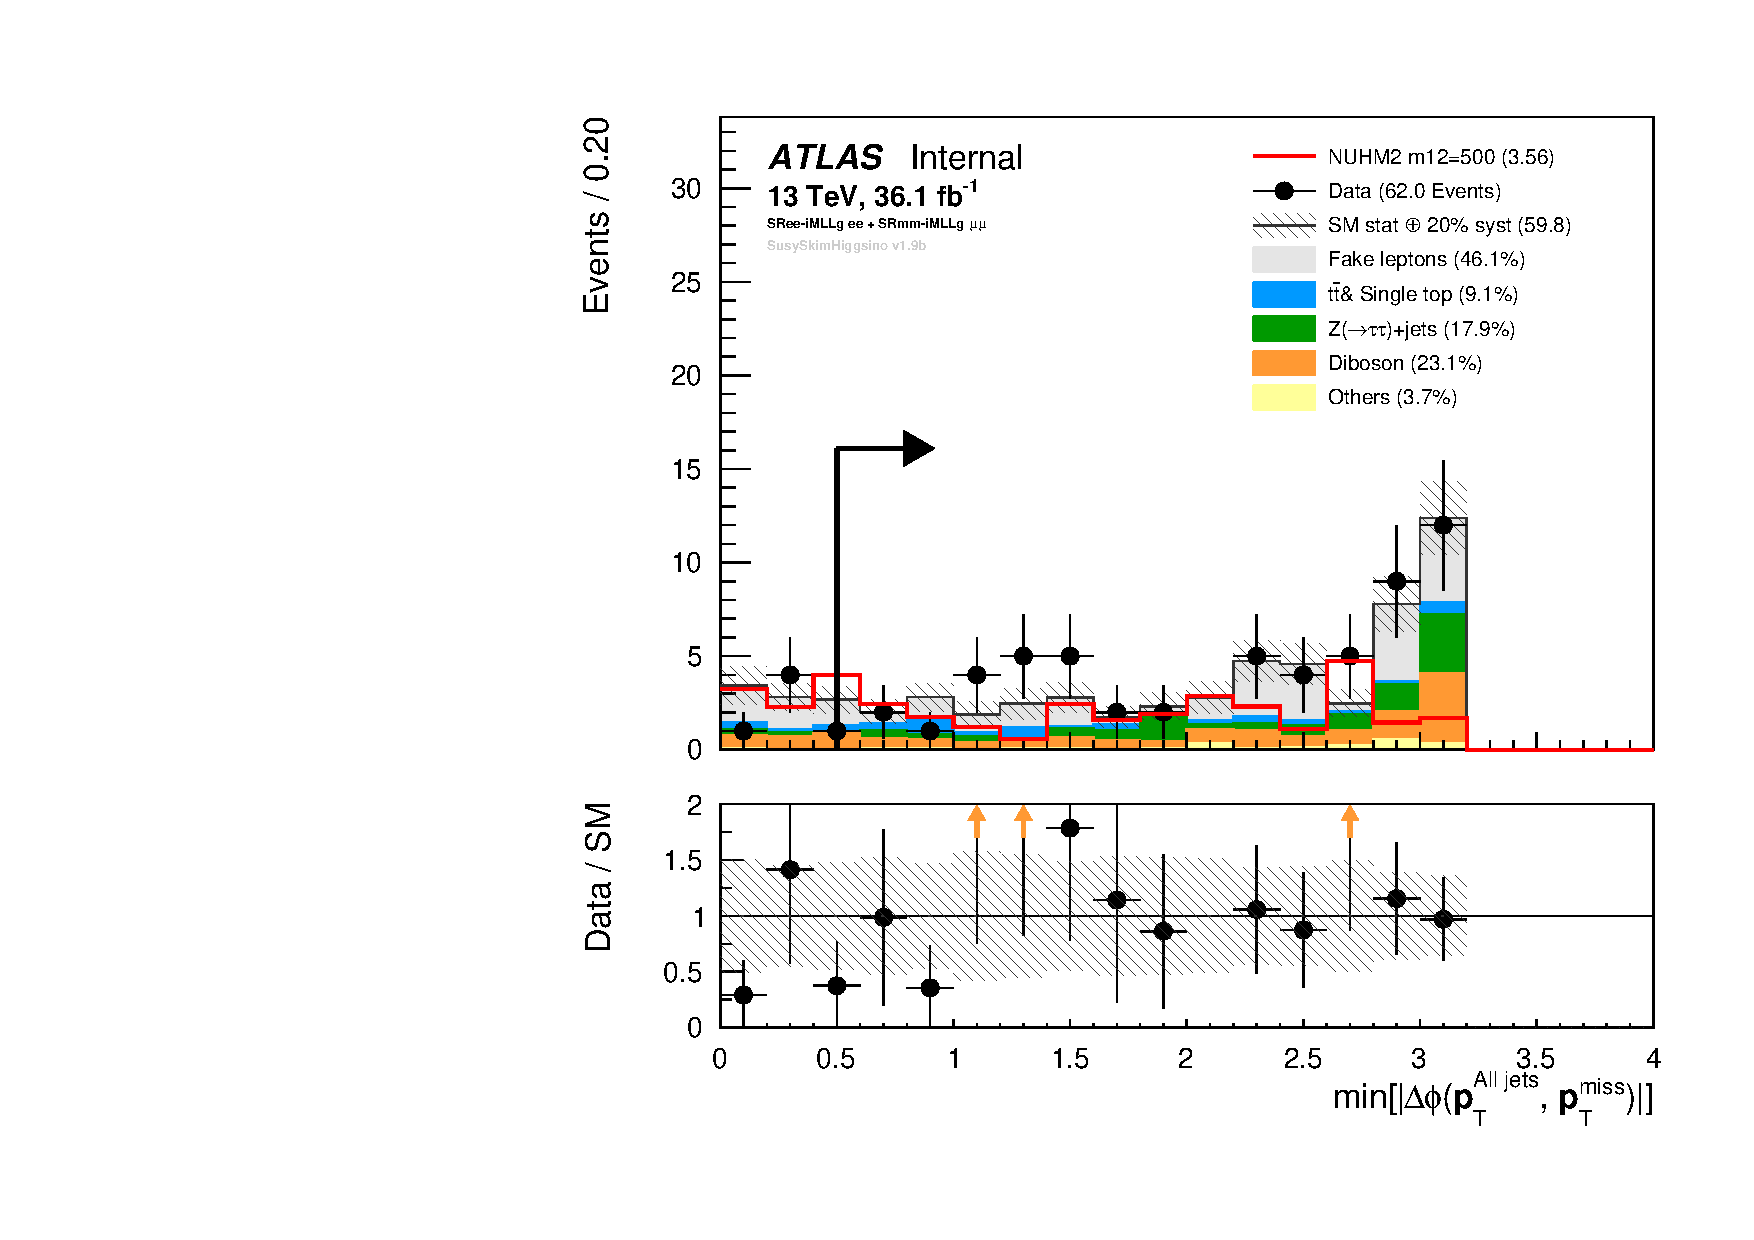
\includegraphics[scale=0.4]{NUHM2_m12_500_and_Bkg_minDPhiAllJetsMet_SFOS_N_minus_one_distribution_in_SR_times_10_on_Nsig.pdf}
            \caption{min[$|\Delta \phi(\mathbf{p}^{\textrm{All jets}}_{\mathrm{T}}, \mathbf{p}^{\mathrm{miss}}_{\mathrm{T}})|$]}
            \label{fig:event_nuhm2_m12_500_minDPhiAllJetsMet_SFOS}
        \end{subfigure}
    \end{center}
    \caption{The `$N-1$' distributions for NUHM2 model with $m_{1/2} = 500$~{\GeV} in SR region $1 < $SR$\ell \ell$-$m_{\ell \ell} < 60$~{\GeV}.
    The NUHM2 distributions are multiplied by 10 but the number of events in the legend use its actual values.
    %The distributions of $m_{\ell \ell}$, $m_{\tau \tau}$, $m_{T}(\ell_{1})$, $\Delta R_{\ell \ell}$, $|\Delta \phi(\mathbf{p}_\mathrm{T}^{j_{1}}, \mathbf{p}_\mathrm{T}^\mathrm{miss})|$, and min[$|\Delta \phi(\mathbf{p}_\mathrm{T}^\mathrm{All\ jets}, \mathbf{p}_\mathrm{T}^\mathrm{miss})|$] are shown.}
    The distributions of $m_{T}(\ell_{1})$, $\Delta R_{\ell \ell}$, $|\Delta \phi(\mathbf{p}_\mathrm{T}^{j_{1}}, \mathbf{p}_\mathrm{T}^\mathrm{miss})|$, and min[$|\Delta \phi(\mathbf{p}_\mathrm{T}^\mathrm{All\ jets}, \mathbf{p}_\mathrm{T}^\mathrm{miss})|$] are shown.}
    \label{fig:event_nuhm2_kinematic_in_SR_SFOS_3}
\end{figure}

%%%
%%%
%%%

\subsubsection{Cutflows}
\label{subsubsec:event_cutflows}
The cutflows is a sequential cumulative yields after the event selections.
Table~\ref{tab:event_cutflow_NUHM2_1} and Table~\ref{tab:event_cutflow_NUHM2_2} shows the signal selection cutflows yield table for the NUHM2 signal with $m_{1/2}$ ranging from 350 to 800~{\GeV}.
The weighted number of events are normalized to 36.1~\ifb and the raw number of events are also shown.

\begin{table}[ht]
    %\begin{center}
    \resizebox{\textwidth}{!}{% <------ Don't forget this %
        %{\tiny
            \begin{tabular}{lllllllllllll}
                \hline
                \hline
                Selection common to all SRs                                                         & \multicolumn{2}{c}{NUHM2 m12=350} & \multicolumn{2}{c}{NUHM2 m12=400} & \multicolumn{2}{c}{NUHM2 m12=500}\\
                                                                                                    & Weighted & Raw                    & Weighted & Raw                    & Weighted & Raw\\
                \hline
                \met triggers, $\met>150$~{\GeV}, $N_\text{baseline}^\ell \geq 2$                   & $205$    & $968$                  & $196$    & $1262$                 & $122.7$  & $1882$\\
                Stau veto                                                                           & $205$    & $968$                  & $196$    & $1262$                 & $122.7$  & $1882$\\
                $N_\text{baseline}^\ell = 2$                                                        & $158$    & $741$                  & $156$    & $975$                  & $96.5$   & $1501$\\
                $N_\text{signal}^\ell = 2$                                                          & $158$    & $741$                  & $156$    & $975$                  & $96.5$   & $1501$\\
                Same flavour                                                                        & $94$     & $445$                  & $100$    & $598$                  & $64.1$   & $1010$\\
                Opposite charge                                                                     & $78$     & $369$                  & $79$     & $503$                  & $55.1$   & $868$\\
                Lepton truth matching                                                               & $78$     & $366$                  & $78$     & $493$                  & $54.0$   & $851$\\
                Lepton author 16 veto                                                               & $77$     & $364$                  & $77$     & $487$                  & $53.8$   & $848$\\
                $\met > 200$~{\GeV}                                                                 & $77$     & $364$                  & $77$     & $487$                  & $53.8$   & $848$\\
                $N_\text{b-jets} = 0$                                                               & $38.0$   & $194$                  & $31.5$   & $234$                  & $22.2$   & $394$\\
                $\pt(j_1) > 100$~{\GeV}                                                             & $38.0$   & $194$                  & $31.5$   & $234$                  & $22.2$   & $394$\\
                $\Delta\phi\left(j_1, \mathbf{p}_\text{T}^\text{miss}\right) > 2.0$                 & $37.3$   & $190$                  & $30.3$   & $223$                  & $21.0$   & $372$\\
                min($\Delta\phi\left(\text{any jet}, \mathbf{p}_\text{T}^\text{miss}\right)) > 0.4$ & $30.7$   & $153$                  & $25.9$   & $188$                  & $17.4$   & $316$\\
                Veto $m_{\tau\tau} \in [0, 160]$~{\GeV}                                             & $26.2$   & $128$                  & $21.6$   & $161$                  & $15.8$   & $287$\\
                $p_\text{T}^{\ell_1} > 5$~{\GeV}                                                    & $26.2$   & $128$                  & $21.6$   & $161$                  & $15.8$   & $287$\\
                $m_{\ell\ell} > 1$~{\GeV}                                                           & $26.2$   & $128$                  & $21.6$   & $161$                  & $15.8$   & $287$\\
                Veto $m_{\ell\ell} \in [3, 3.2]$~{\GeV}                                             & $26.2$   & $128$                  & $21.6$   & $161$                  & $15.7$   & $286$\\
                $m_{\ell\ell} < 60$~{\GeV}                                                          & $26.2$   & $128$                  & $21.6$   & $161$                  & $15.7$   & $286$\\
                $\Delta R_{\ell\ell} > 0.05$~{\GeV}                                                 & $26.2$   & $128$                  & $21.5$   & $160$                  & $15.7$   & $286$\\
                \hline
                SR$\ell\ell$-$m_{\ell\ell}$ selection                                               &          &                        &          &                        &          &\\
                \hline
                $\met / \HT^\text{lep} > \text{max}(5, 15-2\cdot m_{\ell\ell}/\text{GeV})$          & $12.4$   & $60$                   & $9.9$    & $71$                   & $7.9$    & $150$\\
                $\Delta R_{\ell\ell} < 2.0$~{\GeV}                                                  & $6.5$    & $34$                   & $6.7$    & $51$                   & $5.6$    & $105$\\
                $m_\text{T}^{\ell_1} < 70$~{\GeV}                                                   & $2.7$    & $14$                   & $2.5$    & $21$                   & $3.0$    & $52$\\
                %$m_{\ell\ell} < 40$~{\GeV}                                                          & $2.7$    & $14$                   & $2.5$    & $21$                   & $2.9$    & $50$\\
                %$m_{\ell\ell} < 30$~{\GeV}                                                          & $2.2$    & $11$                   & $1.9$    & $15$                   & $2.7$    & $46$\\
                %$m_{\ell\ell} < 20$~{\GeV}                                                          & $1.4$    & $8$                    & $0.66$   & $6$                    & $1.30$   & $27$\\
                %$m_{\ell\ell} < 10$~{\GeV}                                                          & $0.56$   & $3$                    & $0.13$   & $1$                    & $0.37$   & $8$\\
                %$m_{\ell\ell} < 5$~{\GeV}                                                           & $0.0$    & $0$                    & $0.0$    & $0$                    & $0.0$    & $0$\\
                %$m_{\ell\ell} < 3$~{\GeV}                                                           & $0.0$    & $0$                    & $0.0$    & $0$                    & $0.0$    & $0$\\
                \hline
                \hline
            \end{tabular}
        %}
    }
    %\end{center}
    \caption{The yields after the initial preselection and the sequential selections (cutflows) for the SR.
    The weighted number of events are normalized to 36.1~\ifb and the raw number of events are also shown.
    This table only shows $m_{1/2} = 350$, 400, 500~{\GeV}.}
    \label{tab:event_cutflow_NUHM2_1}
\end{table}%

\begin{table}[ht]
    %\begin{center}
    \resizebox{\textwidth}{!}{% <------ Don't forget this %
        %{\tiny
            \begin{tabular}{lllllllllllll}
                \hline
                \hline
                Selection common to all SRs                                                         & \multicolumn{2}{c}{NUHM2 m12=600} & \multicolumn{2}{c}{NUHM2 m12=700} & \multicolumn{2}{c}{NUHM2 m12=800}\\
                                                                                                    & Weighted & Raw                    & Weighted & Raw                    & Weighted & Raw\\
                \hline
                \met triggers, $\met>150$~{\GeV}, $N_\text{baseline}^\ell \geq 2$                   & $76.1$   & $2321$                 & $41.2$   & $2471$                 & $22.2$   & $2500$\\
                Stau veto                                                                           & $76.1$   & $2321$                 & $41.2$   & $2471$                 & $22.2$   & $2500$\\
                $N_\text{baseline}^\ell = 2$                                                        & $63.0$   & $1904$                 & $33.1$   & $1993$                 & $18.1$   & $2029$\\
                $N_\text{signal}^\ell = 2$                                                          & $63.0$   & $1904$                 & $33.1$   & $1993$                 & $18.1$   & $2029$\\
                Same flavour                                                                        & $42.1$   & $1288$                 & $22.7$   & $1383$                 & $12.6$   & $1392$\\
                Opposite charge                                                                     & $35.9$   & $1101$                 & $19.4$   & $1194$                 & $10.9$   & $1205$\\
                Lepton truth matching                                                               & $35.2$   & $1079$                 & $19.1$   & $1174$                 & $10.8$   & $1192$\\
                Lepton author 16 veto                                                               & $35.2$   & $1078$                 & $19.0$   & $1168$                 & $10.8$   & $1189$\\
                $\met > 200$~{\GeV}                                                                 & $35.2$   & $1078$                 & $19.0$   & $1168$                 & $10.8$   & $1189$\\
                $N_\text{b-jets} = 0$                                                               & $13.3$   & $453$                  & $6.8$    & $470$                  & $3.75$   & $477$\\
                $\pt(j_1) > 100$~{\GeV}                                                             & $13.3$   & $453$                  & $6.8$    & $470$                  & $3.75$   & $477$\\
                $\Delta\phi\left(j_1, \mathbf{p}_\text{T}^\text{miss}\right) > 2.0$                 & $12.4$   & $428$                  & $6.5$    & $453$                  & $3.59$   & $455$\\
                min($\Delta\phi\left(\text{any jet}, \mathbf{p}_\text{T}^\text{miss}\right)) > 0.4$ & $10.6$   & $360$                  & $5.47$   & $379$                  & $3.07$   & $383$\\
                Veto $m_{\tau\tau} \in [0, 160]$~{\GeV}                                             & $9.3$    & $315$                  & $4.77$   & $333$                  & $2.73$   & $340$\\
                $p_\text{T}^{\ell_1} > 5$~{\GeV}                                                    & $9.3$    & $315$                  & $4.77$   & $333$                  & $2.73$   & $340$\\
                $m_{\ell\ell} > 1$~{\GeV}                                                           & $9.3$    & $315$                  & $4.76$   & $332$                  & $2.72$   & $339$\\
                Veto $m_{\ell\ell} \in [3, 3.2]$~{\GeV}                                             & $9.3$    & $315$                  & $4.76$   & $332$                  & $2.71$   & $337$\\
                $m_{\ell\ell} < 60$~{\GeV}                                                          & $9.3$    & $315$                  & $4.76$   & $332$                  & $2.71$   & $337$\\
                $\Delta R_{\ell\ell} > 0.05$~{\GeV}                                                 & $9.3$    & $315$                  & $4.76$   & $332$                  & $2.71$   & $337$\\
                \hline
                SR$\ell\ell$-$m_{\ell\ell}$ selection                                               &          &                        &          &                        &          &\\
                \hline
                $\met / \HT^\text{lep} > \text{max}(5, 15-2\cdot m_{\ell\ell}/\text{GeV})$          & $5.5$    & $188$                  & $3.05$   & $226$                  & $1.85$   & $235$\\
                $\Delta R_{\ell\ell} < 2.0$~{\GeV}                                                  & $4.5$    & $153$                  & $2.55$   & $192$                  & $1.47$   & $194$\\
                $m_\text{T}^{\ell_1} < 70$~{\GeV}                                                   & $2.06$   & $78$                   & $1.21$   & $95$                   & $0.64$   & $85$\\
                %$m_{\ell\ell} < 40$~{\GeV}                                                          & $1.99$   & $74$                   & $1.17$   & $92$                   & $0.63$   & $83$\\
                %$m_{\ell\ell} < 30$~{\GeV}                                                          & $1.93$   & $71$                   & $1.14$   & $89$                   & $0.59$   & $78$\\
                %$m_{\ell\ell} < 20$~{\GeV}                                                          & $1.68$   & $61$                   & $1.04$   & $82$                   & $0.56$   & $73$\\
                %$m_{\ell\ell} < 10$~{\GeV}                                                          & $0.47$   & $14$                   & $0.38$   & $32$                   & $0.33$   & $41$\\
                %$m_{\ell\ell} < 5$~{\GeV}                                                           & $0.045$  & $2$                    & $0.070$  & $6$                    & $0.071$  & $8$\\
                %$m_{\ell\ell} < 3$~{\GeV}                                                           & $0.024$  & $1$                    & $0.012$  & $1$                    & $0.045$  & $4$\\
                \hline
                \hline
            \end{tabular}
        %}
    }
    %\end{center}
    \caption{The yields after the initial preselection and the sequential selections (cutflows) for the SR.
    The weighted number of events are normalized to 36.1~\ifb and the raw number of events are also shown.
    This table only shows $m_{1/2} = 600$, 700, 800~{\GeV}.}
    \label{tab:event_cutflow_NUHM2_2}
\end{table}%
